\documentclass[12pt,a4paper]{article}
\usepackage[T1]{fontenc}        % Habilita glifos de 8 bits (essencial para acentos)
\usepackage[utf8]{inputenc}     % Codificação UTF-8
\usepackage[english,brazilian]{babel} % o último idioma continua sendo o principal
\DeclareUnicodeCharacter{00A0}{~} % Trata espaços não quebráveis com segurança
\usepackage[expansion=false]{microtype}
\setlength{\emergencystretch}{3em}
\usepackage{graphicx}
\usepackage{setspace}
\usepackage{indentfirst}
\usepackage[top=3cm, bottom=2cm, left=3cm, right=2cm]{geometry} % Margens padrão ABNT
\usepackage{times}
\usepackage{parskip}
\usepackage{float}
\usepackage{url}
\usepackage{fancyhdr}
\usepackage{fancybox}
\usepackage{amsmath}
\usepackage{booktabs}
\usepackage{xcolor}
\usepackage{listings}
\usepackage{tabularx}
\usepackage{adjustbox}
\usepackage[htt]{hyphenat}
\usepackage{hyperref}
\hypersetup{hidelinks}

\definecolor{codebg}{rgb}{0.96, 0.97, 0.98}
\definecolor{codeborder}{rgb}{0.85, 0.88, 0.92}
\definecolor{codegreen}{rgb}{0.12, 0.55, 0.25}
\definecolor{codeblue}{rgb}{0.10, 0.35, 0.75}
\definecolor{codepurple}{rgb}{0.50, 0.15, 0.65}

\lstdefinestyle{pythonstyle}{
  backgroundcolor=\color{codebg},
  commentstyle=\color{codegreen}\itshape,
  keywordstyle=\color{codeblue}\bfseries,
  stringstyle=\color{codepurple},
  basicstyle=\ttfamily\scriptsize,
  breakatwhitespace=false,
  breaklines=true,
  captionpos=b,
  keepspaces=true,
  numbers=none,
  showspaces=false,
  showstringspaces=false,
  showtabs=false,
  tabsize=2,
  frame=single,
  rulecolor=\color{codeborder},
  extendedchars=true,
  literate=
    {á}{{\'a}}1 {é}{{\'e}}1 {í}{{\'i}}1 {ó}{{\'o}}1 {ú}{{\'u}}1
    {Á}{{\'A}}1 {É}{{\'E}}1 {Í}{{\'I}}1 {Ó}{{\'O}}1 {Ú}{{\'U}}1
    {à}{{\`a}}1 {è}{{\`e}}1 {ì}{{\`i}}1 {ò}{{\`o}}1 {ù}{{\`u}}1
    {ã}{{\~a}}1 {õ}{{\~o}}1 {Ã}{{\~A}}1 {Õ}{{\~O}}1
    {â}{{\^a}}1 {ê}{{\^e}}1 {î}{{\^i}}1 {ô}{{\^o}}1 {û}{{\^u}}1
    {ç}{{\c{c}}}1 {Ç}{{\c{C}}}1
}
\lstset{style=pythonstyle}

\pagestyle{fancy}
\fancyhf{}
\renewcommand{\headrulewidth}{0pt}
\cfoot{\thepage}

\title{\textbf{\normalsize \\[5cm]
RELATÓRIO DO PROJETO 2 \\ ANÁLISE DE TPC-H EM REDIS E CASSANDRA}}
\author{}
\date{}

\begin{document}

% Cabeçalho institucional idêntico ao modelo base
\thisfancyput(35mm,-10mm){
\begin{tabular}{c}
Universidade Tecnológica Federal do Paraná -- \small{UTFPR}\\
Departamento Acadêmico de Informática -- \small{DAINF}\\
Engenharia de Computação \\
ICSB60-S73 -- NoSQL - Bancos de Dados Não Relacionais \\
\\
\end{tabular}}

\maketitle
\begin{center}
\vspace{4.5cm}
\textbf{Vinicius Ferreira Matias} \\[4.5cm]
\textbf{Novembro de 2026}
\end{center}

\newpage

\section*{Introdução}
Este relatório apresenta o projeto de modelagem orientada a consultas, o processo de extração, transformação e carga (ETL), o ciclo iterativo de otimização e a avaliação experimental de desempenho das três primeiras consultas do benchmark TPC-H (Q1, Q2 e Q3) em Fator de Escala 10 ($\text{SF} = 10$, totalizando 59.986.052 registros na tabela \texttt{LINEITEM}) em dois bancos de dados NoSQL de arquiteturas distintas: Redis 7.4 (chave-valor e estruturas de dados em memória RAM) e Apache Cassandra 5.0 (armazenamento distribuído em família de colunas sobre LSM-Tree).

Diferentemente de motores relacionais (MySQL) ou orientados a documentos (MongoDB), que disponibilizam otimizadores declarativos para junções e \textit{pipelines} de agregação no servidor, tanto o Redis quanto o Cassandra exigem modelagem estritamente guiada pelos padrões de acesso das consultas (\textit{Query-Driven Design}), transferindo parte da filtragem secundária, consolidação e ordenação para a camada de aplicação.

Para tentar isolar os gargalos de cada tecnologia, o estudo experimental foi conduzido em três estágios progressivos e validados contra o gabarito relacional do MySQL: (i) Base (1\textsuperscript{a} versão), com implementação direta e conexões centralizadas; (ii) Versão 2 (V2), atuando exclusivamente na camada cliente Python, \textit{parsers} nativos em C (\texttt{hiredis} e \texttt{orjson}) e paralelismo assíncrono no driver, sem alterar o esquema nem recarregar os dados; e (iii) Versão 3 (V3), incorporando \textit{Zone Maps} temporais na Q3 e corrigindo o viés (\textit{skew}) de particionamento de \texttt{o\_orderkey \% 16} no Cassandra via \textit{hash} multiplicativo de Knuth. Nos gráficos das figuras ao final do relatório, essas etapas aparecem rotuladas respectivamente como \textit{Baseline} (\textit{Base}), \textit{Nível 1} (\texttt{N1}) e \textit{Nível 2} (\texttt{N2}).

\section{Estratégia Arquitetural e Modelagem de Dados}

\subsection{Esquema Relacional de Origem (MySQL -- SF=10)}
No ambiente relacional MySQL, a base TPC-H ($\text{SF}=10$) encontra-se normalizada em oito tabelas canônicas (cujas cardinalidades estão listadas na Tabela~\ref{tab:cardinalidades}), atuando como fonte dos dados no processo de ETL e como referência para validação exata em JSON (comparação byte a byte) de todas as saídas produzidas pelo Redis e pelo Cassandra. As consultas Q1, Q2 e Q3 exercitam padrões de acesso complementares sobre esse esquema:

\begin{itemize}
    \item \textbf{Query 1 (\textit{Pricing Summary Report}):} executa varredura massiva sobre \texttt{LINEITEM} com filtro temporal (\texttt{l\_shipdate <= '1998-09-02'}), seis agregações aritméticas (\texttt{SUM}, \texttt{AVG}, \texttt{COUNT}) e agrupamento por \texttt{l\_returnflag} e \texttt{l\_linestatus}.
    \item \textbf{Query 2 (\textit{Minimum Cost Supplier}):} relaciona cinco tabelas (\texttt{PART}, \texttt{PARTSUPP}, \texttt{SUPPLIER}, \texttt{NATION} e \texttt{REGION}) com subconsulta de menor custo regional por peça, filtrando por região, tamanho e sufixo do tipo, retornando as 100 primeiras tuplas ordenadas por saldo (\texttt{s\_acctbal DESC}), país, fornecedor e peça.
    \item \textbf{Query 3 (\textit{Shipping Priority}):} une \texttt{CUSTOMER}, \texttt{ORDERS} e \texttt{LINEITEM} aplicando igualdade de segmento (\texttt{c\_mktsegment = 'BUILDING'}) e duas desigualdades temporais simultâneas (\texttt{o\_orderdate < '1995-03-15'} e \texttt{l\_shipdate > '1995-03-15'}), totalizando pedidos e itens anteriores à data de corte, consolidando o faturamento por pedido e retornando o \textit{top-10}.
\end{itemize}

\begin{table}[H]
\centering
\caption{Cardinalidades verificadas nas tabelas de origem no MySQL ($\text{SF}=10$).}
\label{tab:cardinalidades}
\begin{tabular}{lr}
\toprule
\textbf{Tabela MySQL} & \textbf{Registros Verificados} \\
\midrule
\texttt{REGION}   & 5 \\
\texttt{NATION}   & 25 \\
\texttt{SUPPLIER} & 100.000 \\
\texttt{CUSTOMER} & 1.500.000 \\
\texttt{PART}     & 2.000.000 \\
\texttt{PARTSUPP} & 8.000.000 \\
\texttt{ORDERS}   & 15.000.000 \\
\texttt{LINEITEM} & 59.986.052 \\
\bottomrule
\end{tabular}
\end{table}

\subsection{Decisões Metodológicas para Comparação Justa em SF=10}
Para evitar otimizações assimétricas entre os motores ou acoplamento indevido às propriedades sintéticas do gerador \texttt{dbgen}, quatro diretrizes metodológicas foram estabelecidas:

\begin{enumerate}
    \item \textbf{Q1 -- Pré-agregação diária simétrica:} como a Q1 processa quase a totalidade dos 60 milhões de registros de \texttt{LINEITEM} e filtra unicamente por \texttt{l\_shipdate}, ambos os bancos armazenam agregados diários por \texttt{(l\_shipdate, l\_returnflag, l\_linestatus)} --- exatamente 3.817 linhas --- contendo \texttt{sum\_discount} para derivação exata de \texttt{avg\_disc}. Essa modelagem preserva total flexibilidade para qualquer parâmetro $\Delta$ de corte temporal.
    \item \textbf{Q2 -- Materialização completa das 1.250 combinações em dois modos (\texttt{full} e \texttt{min}):} ambos os bancos carregam integralmente todas as combinações possíveis, aplicando \texttt{LIMIT 100} somente em tempo de consulta. Para quantificar o impacto da pré-computação do mínimo regional no ETL, implementaram-se duas variantes simétricas: \textbf{\texttt{q2\_full}}, que armazena todas as 8.000.000 de ofertas e calcula o mínimo e a ordenação em tempo de consulta; e \textbf{\texttt{q2\_min}}, que pré-filtra via CTE o menor custo regional por peça e já persiste os dados na ordenação exigida.
    \item \textbf{Q3 -- Varredura histórica completa vs. Zone Map:} embora o \texttt{dbgen} do TPC-H garanta $L\_SHIPDATE \le O\_ORDERDATE + 121$ dias, o primeiro caso não explora essa propriedade implícita, percorrendo todo o histórico anterior a 1995-03-15 em ambos os bancos. Já no segundo caso, a poda temporal passa a ser feita por estruturas auxiliares (\textit{Zone Maps}) construídas diretamente a partir do \texttt{MAX(l\_shipdate)} observado nos dados reais.
    \item \textbf{Avaliação do fator de particionamento ($B$) e correção de \textit{skew} na Q3 do Cassandra:} a Q3 desnormalizada foi avaliada com $B \in \{4, 8, 16\}$ usando $\text{bucket} = \text{orderkey} \bmod B$, revelando um viés estrutural nas chaves esparsas do \texttt{dbgen} para $B=16$, posteriormente corrigido por espalhamento via \textit{hash} multiplicativo de Knuth.
\end{enumerate}

\subsection{Modelagem Orientada a Consultas no Apache Cassandra}
No Cassandra, cada consulta e variante foi mapeada em tabelas específicas do \textit{keyspace} \texttt{tpch} (\texttt{SimpleStrategy}, fator de replicação 1), desenhando chaves de partição (\textit{Partition Key}) e colunas de agrupamento (\textit{Clustering Columns}) para suportar consultas de faixa e ordenação sem recorrer a \texttt{ALLOW FILTERING}:

\begin{itemize}
    \item \textbf{\texttt{q1\_daily\_by\_month}:} particionada por \texttt{ship\_month} (\texttt{YYYY-MM}), gerando 84 partições compactas (média de 4,1 KiB) que respondem a filtros de intervalo em \texttt{shipdate}.
    \item \textbf{\texttt{q2\_offers\_by\_filter} (\texttt{q2\_full}):} particionada por \texttt{(region\_name, part\_size, type\_suffix)}, agrupada por \texttt{(partkey ASC, supplycost ASC, suppkey ASC)} para entregar os itens já agrupados por peça e custo crescente à aplicação.
    \item \textbf{\texttt{q2\_min\_offers\_by\_filter} (\texttt{q2\_min}):} mesma chave de partição, porém com \texttt{CLUSTERING ORDER BY (acctbal DESC, nation\_name ASC, supplier\_name ASC, partkey ASC, suppkey ASC)}, permitindo leitura direta em uma única partição com \texttt{LIMIT 100}.
    \item \textbf{\texttt{q3\_lineitems\_by\_segment\_month}:} desnormaliza \texttt{CUSTOMER}, \texttt{ORDERS} e \texttt{LINEITEM} sob chave de partição composta \texttt{(segment, order\_month, bucket)}, ordenando fisicamente por \texttt{order\_date ASC, orderkey ASC, linenumber ASC}.
    \item \textbf{\texttt{q3\_zonemap}:} tabela auxiliar particionada por \texttt{segment} armazenando \texttt{(order\_month, max\_shipdate)} para descartar meses inteiros antes do \textit{scatter-gather}.
\end{itemize}

\begin{lstlisting}[caption={Schemas CQL completos (\texttt{schema.cql} e \texttt{schema\_opt.cql}) utilizados no Apache Cassandra 5.0 ($\text{SF}=10$).}]
CREATE KEYSPACE IF NOT EXISTS tpch
WITH replication = {'class': 'SimpleStrategy', 'replication_factor': 1};
USE tpch;

CREATE TABLE IF NOT EXISTS q1_daily_by_month (
    ship_month text,
    shipdate date,
    returnflag text,
    linestatus text,
    sum_qty decimal,
    sum_base_price decimal,
    sum_disc_price decimal,
    sum_charge decimal,
    sum_discount decimal,
    count_order bigint,
    PRIMARY KEY ((ship_month), shipdate, returnflag, linestatus)
) WITH CLUSTERING ORDER BY (shipdate ASC, returnflag ASC, linestatus ASC);

CREATE TABLE IF NOT EXISTS q2_offers_by_filter (
    region_name text,
    part_size int,
    type_suffix text,
    partkey int,
    supplycost decimal,
    suppkey int,
    acctbal decimal,
    supplier_name text,
    nation_name text,
    mfgr text,
    address text,
    phone text,
    supplier_comment text,
    PRIMARY KEY ((region_name, part_size, type_suffix), partkey, supplycost, suppkey)
) WITH CLUSTERING ORDER BY (partkey ASC, supplycost ASC, suppkey ASC);

CREATE TABLE IF NOT EXISTS q2_min_offers_by_filter (
    region_name text,
    part_size int,
    type_suffix text,
    acctbal decimal,
    nation_name text,
    supplier_name text,
    partkey int,
    suppkey int,
    mfgr text,
    address text,
    phone text,
    supplier_comment text,
    supplycost decimal,
    PRIMARY KEY ((region_name, part_size, type_suffix), acctbal, nation_name, supplier_name, partkey, suppkey)
) WITH CLUSTERING ORDER BY (acctbal DESC, nation_name ASC, supplier_name ASC, partkey ASC, suppkey ASC);

CREATE TABLE IF NOT EXISTS q3_lineitems_by_segment_month (
    segment text,
    order_month text,
    bucket int,
    order_date date,
    orderkey bigint,
    linenumber int,
    shipdate date,
    shippriority int,
    extendedprice decimal,
    discount decimal,
    PRIMARY KEY ((segment, order_month, bucket), order_date, orderkey, linenumber)
) WITH CLUSTERING ORDER BY (order_date ASC, orderkey ASC, linenumber ASC);

-- Extensao (schema_opt.cql):
CREATE TABLE IF NOT EXISTS q3_zonemap (
    segment text,
    order_month text,
    max_shipdate date,
    PRIMARY KEY ((segment), order_month)
) WITH CLUSTERING ORDER BY (order_month ASC);
\end{lstlisting}

\subsection{Modelagem de Estruturas em Memória no Redis}
Para manter os dados de $\text{SF}=10$ dentro do teto de 7 GB no Redis sem explosão de metadados no dicionário global de chaves, cada consulta utilizou estruturas compactas definidas em \texttt{common/codecs.py}:

\begin{itemize}
    \item \textbf{Q1 (\texttt{ZSET} + \texttt{HASH} diário):} um \texttt{ZSET} (\texttt{tpch:q1:days}) indexa as datas disponíveis usando \texttt{score = YYYYMMDD}. Cada dia aponta para um único \texttt{HASH} (\texttt{tpch:q1:day:\{YYYY-MM-DD\}}) cujos campos são os pares \texttt{\{returnflag\}|\{linestatus\}} e os valores são os seis acumuladores concatenados por \texttt{|}, totalizando apenas 2,12 MiB em RAM.
    \item \textbf{Q2 (\texttt{LIST} por combinação):} para cada uma das combinações, o modo \texttt{full} armazena todas as ofertas na lista \texttt{tpch:q2:offers:\{R\}:\{S\}:\{T\}} (1,49 GiB), enquanto o modo \texttt{min} armazena apenas as ofertas mínimas já ordenadas em \texttt{tpch:q2:min:\{R\}:\{S\}:\{T\}} (1,10 GiB), permitindo resposta em um único \texttt{LRANGE 0 99}.
    \item \textbf{Q3 (\texttt{HASH} diário com \textit{payload} binário \texttt{struct}):} em vez de criar dezenas de milhões de chaves individuais por pedido ou item, as datas de cada segmento são indexadas no \texttt{ZSET} \texttt{tpch:q3:days:\{SEGMENT\}} e todos os pedidos de um mesmo dia e segmento são agrupados em um \texttt{HASH} diário \texttt{tpch:q3:day:\{SEGMENT\}:\{YYYY-MM-DD\}} (cerca de 12.030 chaves no total). Cada campo do \textit{hash} corresponde ao \texttt{orderkey} e seu valor é um registro binário compacto empacotado com \texttt{struct} (\texttt{<iH} para \texttt{shippriority} e contagem de itens, seguido de $n$ registros \texttt{<IqH} contendo \texttt{shipdate} em inteiro, \texttt{extendedprice * 100} e \texttt{discount * 100}), consumindo apenas 1,72 GiB para os 15 milhões de pedidos e 59,99 milhões de itens.
    \item \textbf{Q3 Zone Map:} cinco \texttt{HASH}es auxiliares \texttt{tpch:q3:zonemap:\{SEGMENT\}} mapeiam cada \texttt{YYYY-MM-DD} ao respectivo \texttt{MAX(l\_shipdate)} inteiro (12.030 entradas, acréscimo de apenas +783,0 KiB sobre o snapshot da Q3).
\end{itemize}

\begin{lstlisting}[language=Python, caption={Codec binário compacto da Q3 e convenção de chaves em \texttt{common/codecs.py}.}]
import struct

ORDER_HDR = struct.Struct("<iH")   # shippriority (int32), n_items (uint16)
ITEM_REC  = struct.Struct("<IqH")  # shipdate_int (uint32), ext_cents (uint64), disc_pct (uint16)

def pack_q3_order(shippriority: int, items: list[tuple[int, int, int]]) -> bytes:
    buf = bytearray(ORDER_HDR.pack(shippriority, len(items)))
    for it in items:
        buf.extend(ITEM_REC.pack(*it))
    return bytes(buf)

def calc_q3_order_revenue(blob: bytes, cutoff_int: int) -> tuple[int, int]:
    sprio, n_items = ORDER_HDR.unpack_from(blob, 0)
    rev_1e4 = 0
    offset = ORDER_HDR.size
    for _ in range(n_items):
        sdate_int, ext_c, disc_h = ITEM_REC.unpack_from(blob, offset)
        offset += ITEM_REC.size
        if sdate_int > cutoff_int:
            rev_1e4 += ext_c * (100 - disc_h)
    return sprio, rev_1e4
\end{lstlisting}

\subsection{Processo de ETL, Centralização de Conexões e Carga em Escala SF=10}
Para suportar o volume do $\text{SF}=10$ sem esgotamento de memória ou quedas silenciosas de conexão durante janelas longas de processamento, o módulo compartilhado \texttt{common/config.py} centralizou toda a resolução dinâmica de caminhos (\texttt{BASE\_DIR} relativo ao arquivo, independente de \texttt{\$HOME}) e as fábricas de conexão parametrizáveis por variáveis de ambiente:

\begin{enumerate}
    \item \textbf{Controle centralizado de timeouts:} \texttt{get\_mysql\_conn()} ajusta automaticamente \texttt{net\_write\_timeout = 600} e \texttt{net\_read\_timeout = 600} na sessão para evitar \textit{Lost connection to MySQL server (2013)} durante a carga da Q3; \texttt{get\_cassandra\_session()} configura \texttt{default\_timeout = 120.0} s e \texttt{default\_fetch\_size = 10000} (sobrescritos para \texttt{50000} nos testes otimizados); e \texttt{get\_redis\_client()} padroniza o acesso ao cliente RESP.
    \item \textbf{Extração fatiada e publicação atômica na Q2 (25 fatias):} para evitar tabelas temporárias gigantes no MySQL ao cruzar 8 milhões de linhas de \texttt{PARTSUPP}, a carga da Q2 é particionada em 25 fatias independentes ($5 \text{ regiões} \times 5 \text{ sufixos}$). No Redis, cada fatia é escrita em 50 chaves temporárias (\texttt{tmp:...}) e publicada atomicamente em bloco \texttt{MULTI/EXEC} (\texttt{RENAME}/\texttt{DEL}); no Cassandra, as inserções ocorrem via \texttt{execute\_concurrent\_with\_args} com \texttt{concurrency=64}.
    \item \textbf{Exportação paralela para CSV e \textit{rebucketing} local da Q3:} em \texttt{Cassandra/load/export\_q3\_csv.py}, cinco processos paralelos (\texttt{ProcessPoolExecutor}) extraem cada segmento em janelas anuais (\texttt{1992..1998}) usando cursor \texttt{raw=True} do MySQL e gravação em bytes com buffer de 1 MiB, reduzindo a exportação inicial dos 59.986.052 registros (\texttt{b=4}) para 166,56 s. Para as variações \texttt{b=8}, \texttt{b=16 mod} e \texttt{b=16 hash}, a opção \texttt{--from-buckets 4} lê os CSVs locais e recalcula apenas a coluna \texttt{bucket}, concluindo em 9,33 s a 10,09 s sem reconsultar o MySQL.
    \item \textbf{Ingestão em massa via DSBulk 1.11.0:} o script \texttt{Cassandra/load/load\_q3\_dsbulk.sh} valida os cabeçalhos dos cinco CSVs, trunca a tabela alvo, limpa snapshots anteriores e executa o DataStax Bulk Loader (\texttt{dsbulk load}) processando os cinco arquivos em paralelo (\texttt{-maxConcurrentFiles 5}, \texttt{-maxConcurrentQueries 64}, \texttt{--driver.basic.request.timeout "60 seconds"}), atingindo vazão sustentada de 204 mil a 237 mil escritas/s com 0 falhas em todas as rodadas.
    \item \textbf{Carga paralela dos Zone Maps:} os scripts \texttt{load\_q3\_zonemap.py} (Redis e Cassandra) utilizam 5 processos paralelos por segmento e janelas anuais no MySQL (\texttt{GROUP BY o.o\_orderdate}), consolidando o índice auxiliar em $\sim$671--673 s (com escrita efetiva no banco em apenas 20 ms no Redis e 47 ms no Cassandra).
\end{enumerate}

\begin{lstlisting}[caption={Consulta CTE fatiada da Q2 (\texttt{load\_q2.py}) e ingestão paralela via DSBulk (\texttt{load\_q3\_dsbulk.sh}).}]
-- Extracao segura de uma fatia (regiao x sufixo) da Q2 no MySQL (modo min):
WITH min_cost AS (
    SELECT ps.ps_partkey, MIN(ps.ps_supplycost) AS min_sc
    FROM PARTSUPP ps
    JOIN SUPPLIER s ON s.s_suppkey = ps.ps_suppkey
    JOIN NATION n   ON n.n_nationkey = s.s_nationkey
    JOIN REGION r   ON r.r_regionkey = n.n_regionkey
    WHERE r.r_name = %s
    GROUP BY ps.ps_partkey
)
SELECT
    p.p_size, p.p_partkey, ps.ps_supplycost, s.s_suppkey,
    s.s_acctbal, n.n_name, s.s_name, p.p_mfgr,
    s.s_address, s.s_phone, s.s_comment
FROM PART p
JOIN PARTSUPP ps ON ps.ps_partkey = p.p_partkey
JOIN min_cost mc ON mc.ps_partkey = ps.ps_partkey
                AND mc.min_sc = ps.ps_supplycost
JOIN SUPPLIER s  ON s.s_suppkey = ps.ps_suppkey
JOIN NATION n    ON n.n_nationkey = s.s_nationkey
JOIN REGION r    ON r.r_regionkey = n.n_regionkey
WHERE r.r_name = %s AND p.p_type LIKE CONCAT('%', %s)
ORDER BY s.s_acctbal DESC, n.n_name ASC, s.s_name ASC, p.p_partkey ASC, s.s_suppkey ASC;

# Ingestao paralela dos 5 CSVs da Q3 no Cassandra via DSBulk 1.11.0:
dsbulk load \
    -h 127.0.0.1 -k tpch -t q3_lineitems_by_segment_month \
    -url "$CSV_DIR" -maxConcurrentFiles 5 -header true \
    --schema.mapping "$MAPPING" \
    --driver.basic.request.timeout "$DSBULK_TIMEOUT" \
    -maxConcurrentQueries "$DSBULK_CONCURRENCY" \
    -logDir "$OUT_DIR/dsbulk_logs_${SUFFIX}"
\end{lstlisting}

\subsection{Arquitetura dos Contêineres, Hardware e Controle Experimental}
Todos os experimentos foram executados na mesma máquina hospedeira Linux (Ubuntu 22.04.5 LTS), equipada com processador AMD Ryzen 7 7735HS (8 núcleos / 16 \textit{threads}), 30 GiB de memória RAM disponíveis e swap desativado (\texttt{0 B}). Para garantir isolamento de recursos, os contêineres \texttt{tpch\_redis} e \texttt{tpch\_cassandra} foram executados de forma mutuamente exclusiva via Docker Compose:

\begin{enumerate}
    \item \textbf{Apache Cassandra 5.0 (\textit{Heap}, \textit{Cgroup} e \textit{Timeouts}):} o contêiner foi limitado a \texttt{mem\_limit: 6g} e \texttt{memswap\_limit: 6g}, com a JVM ajustada para \texttt{MAX\_HEAP\_SIZE=3G} e \texttt{HEAP\_NEWSIZE=768M} (reduzindo pausas de \textit{Garbage Collector} durante o \texttt{dsbulk load} e reservando cerca de 3 GiB para \textit{Page Cache} das SSTables). Montou-se um arquivo \texttt{cassandra.yaml} personalizado com \texttt{read\_request\_timeout: 30s}, \texttt{range\_request\_timeout: 30s}, \texttt{write\_request\_timeout: 15s}, \texttt{request\_timeout: 30s} e \texttt{truncate\_request\_timeout: 60000ms}. Após cada carga, executou-se \texttt{nodetool flush tpch} antes de coletar \texttt{tablestats} e \texttt{tablehistograms}.
    \item \textbf{Redis 7.4 (Isolamento por Consulta e Snapshots RDB):} desativaram-se RDB automático e AOF (\texttt{--save "" --appendonly no}) e configurou-se \texttt{--maxmemory 7gb --maxmemory-policy noeviction} (\texttt{mem\_limit: 8g}, \texttt{mem\_swappiness: 0}). Cada consulta (\texttt{q1}, \texttt{q2\_full}, \texttt{q2\_min}, \texttt{q3} e \texttt{q3\_zonemap}) foi carregada isoladamente após \texttt{--flush}, preservada via \texttt{redis-cli SAVE} síncrono em \texttt{redis\_backups/*.rdb} e restaurada em contêiner limpo antes das baterias de teste, registrando \texttt{INFO memory} após cada carga.
\end{enumerate}

\begin{lstlisting}[caption={Configuração do \texttt{docker-compose.yml} e comandos operacionais de consolidação e coleta.}]
services:
  redis:
    image: redis:7.4-alpine
    container_name: tpch_redis
    ports:
      - "6379:6379"
    command: >
      redis-server --save "" --appendonly no
      --maxmemory 7gb --maxmemory-policy noeviction
    volumes:
      - ./redis_data:/data
    mem_limit: 8g
    memswap_limit: 8g
    mem_swappiness: 0

  cassandra:
    image: cassandra:5.0
    container_name: tpch_cassandra
    ports:
      - "9042:9042"
    environment:
      - CASSANDRA_CLUSTER_NAME=tpch_cluster
      - MAX_HEAP_SIZE=3G
      - HEAP_NEWSIZE=768M
    volumes:
      - ./cassandra_data:/var/lib/cassandra
      - ./cassandra.yaml:/etc/cassandra/cassandra.yaml
    mem_limit: 6g
    memswap_limit: 6g

# Consolidacao fisica e estatisticas no Cassandra pos-carga:
docker exec tpch_cassandra nodetool flush tpch q3_lineitems_by_segment_month
docker exec tpch_cassandra nodetool tablestats tpch.q3_lineitems_by_segment_month > results/tablestats_q3_b16_hash.txt
docker exec tpch_cassandra nodetool tablehistograms tpch q3_lineitems_by_segment_month > results/tablehistograms_q3_b16_hash.txt

# Snapshot sincrono e inspecao de memoria no Redis:
docker exec tpch_redis redis-cli SAVE
docker exec tpch_redis redis-cli INFO memory
\end{lstlisting}

\newpage

\section{Equivalência de Consultas e Estratégias de Otimização}

Esta seção apresenta as consultas SQL de referência no MySQL (\texttt{mysql\_result.py}), o fluxo de comandos equivalente no Redis e no Cassandra e as otimizações implementadas nas Versões 2 e 3.

\subsection{Consultas SQL de Referência (MySQL)}

\begin{lstlisting}[caption={Queries 1, 2 e 3 executadas no MySQL como gabarito (\textit{ground truth}) em \texttt{mysql\_result.py}.}]
-- QUERY 1: Pricing Summary Report (delta = 90 dias -> 1998-09-02)
SELECT l_returnflag, l_linestatus,
    SUM(l_quantity), SUM(l_extendedprice),
    SUM(l_extendedprice * (1 - l_discount)),
    SUM(l_extendedprice * (1 - l_discount) * (1 + l_tax)),
    AVG(l_quantity), AVG(l_extendedprice), AVG(l_discount), COUNT(*)
FROM LINEITEM
WHERE l_shipdate <= '1998-09-02'
GROUP BY l_returnflag, l_linestatus
ORDER BY l_returnflag, l_linestatus;

-- QUERY 2: Minimum Cost Supplier (EUROPE / 15 / BRASS)
WITH min_cost AS (
    SELECT ps.ps_partkey, MIN(ps.ps_supplycost) AS min_sc
    FROM PARTSUPP ps
    JOIN SUPPLIER s ON s.s_suppkey = ps.ps_suppkey
    JOIN NATION n   ON n.n_nationkey = s.s_nationkey
    JOIN REGION r   ON r.r_regionkey = n.n_regionkey
    WHERE r.r_name = 'EUROPE'
    GROUP BY ps.ps_partkey
)
SELECT s.s_acctbal, s.s_name, n.n_name, p.p_partkey,
       p.p_mfgr, s.s_address, s.s_phone, s.s_comment
FROM PART p
JOIN PARTSUPP ps ON ps.ps_partkey = p.p_partkey
JOIN min_cost mc ON mc.ps_partkey = ps.ps_partkey AND mc.min_sc = ps.ps_supplycost
JOIN SUPPLIER s  ON s.s_suppkey = ps.ps_suppkey
JOIN NATION n    ON n.n_nationkey = s.s_nationkey
JOIN REGION r    ON r.r_regionkey = n.n_regionkey
WHERE p.p_size = 15 AND p.p_type LIKE '%BRASS' AND r.r_name = 'EUROPE'
ORDER BY s.s_acctbal DESC, n.n_name ASC, s.s_name ASC, p.p_partkey ASC
LIMIT 100;

-- QUERY 3: Shipping Priority (BUILDING / 1995-03-15)
SELECT l.l_orderkey, SUM(l.l_extendedprice * (1 - l.l_discount)) AS revenue,
       o.o_orderdate, o.o_shippriority
FROM CUSTOMER c
JOIN ORDERS o   ON c.c_custkey = o.o_custkey
JOIN LINEITEM l ON l.l_orderkey = o.o_orderkey
WHERE c.c_mktsegment = 'BUILDING'
  AND o.o_orderdate < '1995-03-15'
  AND l.l_shipdate > '1995-03-15'
GROUP BY l.l_orderkey, o.o_orderdate, o.o_shippriority
ORDER BY revenue DESC, o.o_orderdate ASC
LIMIT 10;
\end{lstlisting}

\subsection{Fluxo de Execução no Redis}

\begin{lstlisting}[caption={Sequência de comandos Redis executados para Q1, Q2 (\texttt{full}/\texttt{min}), Q3 e Q3 Zone Map.}]
# QUERY 1: Filtro temporal no ZSET e leitura em pipeline dos HASHes diarios
ZRANGEBYSCORE tpch:q1:days -inf 19980902
# Em pipeline (transaction=False):
HGETALL tpch:q1:day:{YYYY-MM-DD}           # soma acumuladores e deriva medias em Python

# QUERY 2 (full vs min):
LRANGE tpch:q2:offers:EUROPE:15:BRASS 0 -1 # full: agrupa min(supplycost) e ordena top-100 no cliente
LRANGE tpch:q2:min:EUROPE:15:BRASS 0 99    # min:  leitura direta das 100 primeiras ofertas ordenadas

# QUERY 3 (Base / V2) e Q3 + Zone Map (V3):
ZRANGEBYSCORE tpch:q3:days:BUILDING -inf (19950315
HGETALL tpch:q3:zonemap:BUILDING           # apenas na versao 3: poda dias com max_shipdate <= 19950315
# Em pipeline em lotes (30 dias na Base; 60 dias na V2/V3):
HGETALL tpch:q3:day:BUILDING:{YYYY-MM-DD}  # desempacota payload binario, filtra shipdate > 19950315
                                           # e seleciona top-10 via heapq.nsmallest no cliente
\end{lstlisting}

\subsection{Consultas CQL no Apache Cassandra}

\begin{lstlisting}[caption={Consultas CQL preparadas executadas no Apache Cassandra para Q1, Q2, Q3 e Zone Map.}]
-- QUERY 1: Executada para todos os meses <= '1998-09' (sequencial na Base; async na V2)
SELECT returnflag, linestatus, sum_qty, sum_base_price,
       sum_disc_price, sum_charge, sum_discount, count_order
FROM q1_daily_by_month
WHERE ship_month = ? AND shipdate <= ?;

-- QUERY 2 (modo full vs modo min):
SELECT partkey, supplycost, suppkey, acctbal, supplier_name, nation_name,
       mfgr, address, phone, supplier_comment
FROM q2_offers_by_filter
WHERE region_name = ? AND part_size = ? AND type_suffix = ?;

SELECT acctbal, supplier_name, nation_name, partkey, mfgr, address, phone,
       supplier_comment
FROM q2_min_offers_by_filter
WHERE region_name = ? AND part_size = ? AND type_suffix = ? LIMIT 100;

-- QUERY 3 (Versao 3 consulta q3_zonemap antes para filtrar apenas meses com max_shipdate > cutoff):
SELECT order_month, max_shipdate FROM q3_zonemap WHERE segment = ?;

SELECT order_date, orderkey, shipdate, shippriority, extendedprice, discount
FROM q3_lineitems_by_segment_month
WHERE segment = ? AND order_month = ? AND bucket = ? AND order_date < ?;
\end{lstlisting}

\subsection{Otimizações Implementadas}
Com a primeira rodada de testes (Base) validada e preservada em \texttt{results\_baseline/}, aplicaram-se duas etapas independentes de otimização (Versão 2 e Versão 3):

\subsubsection*{Versão 2 (V2) --- Camada Cliente, Parsers em C e Paralelismo (sem alteração nos dados)}
\begin{itemize}
    \item \textbf{Redis (\texttt{Redis/opt/test\_q*\_opt.py}):} instalou-se \texttt{hiredis 3.5.0} (substituindo o parser RESP em Python puro por extensão em C) e \texttt{orjson 3.13.0} na \texttt{.venv}. Na Q2 \texttt{full}, a ordenação passou a comparar \texttt{float} em vez de instanciar \texttt{Decimal} por tupla --- seguro porque os campos TPC-H têm 2 casas decimais e no máximo 6 dígitos significativos ($[-999{,}99;\; 9999{,}99]$), preservados exatamente pela mantissa de 53 bits do IEEE-754 \textit{double}, mantendo \texttt{q\_dec} na saída final. Na Q3, o \textit{pipeline} foi ampliado para blocos de 60 dias, adotou-se decodificação tardia (\textit{lazy decode}) da chave de data somente para pedidos aprovados e pré-compilaram-se objetos \texttt{struct.Struct} para desempacotar de 1 a 7 itens em uma única chamada \texttt{unpack\_from}.
    \item \textbf{Cassandra (\texttt{Cassandra/opt/test\_q*\_opt.py}):} substituiu-se o \textit{row factory} padrão (\texttt{namedtuple}) por \texttt{tuple\_factory}; elevou-se \texttt{fetch\_size} para \texttt{50000}; paralelizaram-se as leituras por partição via \texttt{session.execute\_async} em janelas concorrentes (\texttt{concurrency=32} na Q1 para os 81 meses; \texttt{concurrency=16} na Q3 para $\text{meses} \times B$); e na Q3 eliminaram-se alocações \texttt{datetime.date} comparando diretamente \texttt{sdate.days\_from\_epoch > cutoff\_days} (com cache de conversão ISO de \texttt{order\_date}). Como toda soma usa \texttt{Decimal}/\texttt{int} exatos, a execução fora de ordem entre partições é matematicamente comutativa e associativa.
\end{itemize}

\subsubsection*{Versão 3 (V3) --- Zone Maps na Q3 e Correção de \textit{Skew} (sem scripts Lua no Redis)}
\begin{itemize}
    \item \textbf{Poda temporal por Zone Map:} para o predicado \texttt{o\_orderdate < 1995-03-15} e \texttt{l\_shipdate > 1995-03-15} no segmento \texttt{BUILDING}, o Zone Map diário do Redis (\texttt{tpch:q3:zonemap:BUILDING}) e o Zone Map mensal do Cassandra (\texttt{tpch.q3\_zonemap}) permitem podar parte dos dados históricos antes da varredura principal, descartando dias e meses cujo maior \texttt{l\_shipdate} não ultrapassa a data de corte.
    \item \textbf{Uniformização de partições com Hash de Knuth:} ao diagnosticar que o operador módulo simples (\texttt{orderkey \% 16}) deixava metade dos \textit{buckets} completamente vazios no TPC-H, implementou-se (\texttt{--bucket-mode hash}) a dispersão \texttt{((orderkey * 2654435761) >> 16) \% 16}, distribuindo uniformemente todas as 16 classes de partição.
    \item \textbf{Dispensa intencional de Lua no Redis:} optou-se por não mover o cálculo da Q3 para scripts Lua no servidor Redis porque a execução Lua bloqueia o \textit{event loop single-threaded} da instância durante toda a varredura, ao passo que a combinação de \texttt{hiredis} + Zone Map no cliente já atingiu 195,45 ms sem bloquear requisições concorrentes.
\end{itemize}

\newpage

\section{Evidências de Execução, Instrumentação e Análise de Desempenho}

\subsection{Instrumentação de Benchmark e Validação de Integridade}
Todas as medições de latência foram realizadas pelo executor centralizado \texttt{common/test\_runner.py} utilizando \texttt{time.perf\_counter()} em milissegundos, decompondo cada execução em \texttt{t\_db\_ms} (rede, \textit{pipeline}/CQL, paginação e \textit{parsing} do driver), \texttt{t\_app\_ms} (filtragem, desempacotamento, agregação e ordenação em Python) e \texttt{t\_total\_ms}. Adotou-se o protocolo de 3 \textit{warm-ups} e 30 repetições medidas para Q1, Q2 (\texttt{full}/\texttt{min}) e Q3 com Zone Map no Redis, e 1 \textit{warm-up} com 3 repetições nos cenários extensos da Q3 sem poda ou no Cassandra.

\begin{lstlisting}[language=Python, caption={Instrumentação centralizada e gravação automática de saídas para auditoria em \texttt{common/test\_runner.py}.}]
def run_test(
    db_name: str, query_name: str, exec_fn,
    warmup: int, repeat: int, validate: bool,
    extra_meta: dict | None = None, filename_suffix: str = "",
):
    warmup_runs = []
    res = []
    for _ in range(warmup):
        res, m = exec_fn()
        warmup_runs.append(m)

    measured_runs = []
    for _ in range(repeat):
        res, m = exec_fn()
        measured_runs.append(m)

    valid = None
    if validate:
        ref_file = "ref_q2.json" if query_name.startswith("q2") else f"ref_{query_name}.json"
        with open(RESULTS_DIR / ref_file, encoding="utf-8") as f:
            ref = json.load(f)
        valid = (res == ref)

    out_rows_path = RESULTS_DIR / f"output_{db_name}_{query_name}{filename_suffix}.json"
    save_json(out_rows_path, res)  # gravado fora da janela medida
    # ... salva payload JSON com resumo estatistico (mean, median, stdev, min, max)
\end{lstlisting}

Após a conclusão de todas as baterias, a auditoria automatizada (\texttt{generate\_report.py}) confirmou que todos os arquivos \texttt{output\_*.json} são idênticos byte a byte às referências \texttt{ref\_q1.json}, \texttt{ref\_q2.json} e \texttt{ref\_q3.json}. A Tabela~\ref{tab:amostra_gabarito} registra os valores exatos validados na Q1 e os cinco primeiros pedidos da Q3.

\begin{table}[H]
\centering
\small
\setlength{\tabcolsep}{4pt}
\caption{Amostra exata das saídas validadas contra o MySQL (\texttt{ref\_q1.json} e \texttt{ref\_q3.json}, $\text{SF}=10$).}
\label{tab:amostra_gabarito}
\begin{adjustbox}{max width=\textwidth}
\begin{tabular}{ccccrrrr}
\toprule
\multicolumn{8}{c}{\textbf{Query 1 --- 4 grupos retornados (59.142.609 itens somados)}} \\
\midrule
\textbf{\texttt{flag}} & \textbf{\texttt{status}} & \textbf{\shortstack[c]{\texttt{count\_}\\\texttt{order}}} & \textbf{\shortstack[c]{\texttt{sum\_}\\\texttt{qty}}} & \textbf{\shortstack[r]{\texttt{sum\_base\_}\\\texttt{price}}} & \textbf{\shortstack[r]{\texttt{sum\_disc\_}\\\texttt{price}}} & \textbf{\shortstack[r]{\texttt{avg\_}\\\texttt{price}}} & \textbf{\shortstack[r]{\texttt{avg\_}\\\texttt{disc}}} \\
\midrule
A & F & 14.804.077 & 377.518.399,00 & 566.065.727.797,25 & 537.759.104.278,0656 & 38.237,1510 & 0,0500 \\
N & F &    385.998 &   9.851.614,00 &  14.767.438.399,17 &  14.028.805.792,2114 & 38.257,8107 & 0,0500 \\
N & O & 29.144.351 & 743.124.873,00 & 1.114.302.286.901,88 & 1.058.580.922.144,9638 & 38.233,9029 & 0,0500 \\
R & F & 14.808.183 & 377.732.830,00 & 566.431.054.976,00 & 538.110.922.664,7677 & 38.251,2193 & 0,0500 \\
\midrule
\multicolumn{8}{c}{\textbf{Query 3 --- Primeiros 5 pedidos do \textit{Top-10} (\texttt{BUILDING}, corte \texttt{1995-03-15})}} \\
\midrule
\multicolumn{2}{c}{\textbf{Rank}} & \textbf{\texttt{orderkey}} & \textbf{\texttt{orderdate}} & \textbf{\texttt{shippriority}} & \multicolumn{3}{r}{\textbf{\texttt{revenue} (114.003 pedidos válidos)}} \\
\midrule
\multicolumn{2}{c}{1} & 4.791.171  & 1995-02-23 & 0 & \multicolumn{3}{r}{440.715,2185} \\
\multicolumn{2}{c}{2} & 46.678.469 & 1995-01-27 & 0 & \multicolumn{3}{r}{439.855,3250} \\
\multicolumn{2}{c}{3} & 23.906.758 & 1995-03-14 & 0 & \multicolumn{3}{r}{432.728,5737} \\
\multicolumn{2}{c}{4} & 23.861.382 & 1995-03-09 & 0 & \multicolumn{3}{r}{428.739,1368} \\
\multicolumn{2}{c}{5} & 59.393.639 & 1995-02-12 & 0 & \multicolumn{3}{r}{426.036,0662} \\
\bottomrule
\end{tabular}
\end{adjustbox}
\end{table}


\subsection{Consolidação dos Custos de Carga (ETL) e Armazenamento}
As Tabelas~\ref{tab:carga_etl}, \ref{tab:redis_mem} e \ref{tab:cass_disco} consolidam, respectivamente, os tempos de extração/transformação/carga nos 13 cenários de ETL, o consumo de RAM no Redis (\texttt{INFO memory}) e o espaço físico em disco no Cassandra pós-\texttt{nodetool flush} (\texttt{nodetool tablestats}). Esses dados encontram-se ilustrados nas Figuras~\ref{fig:redis_mem_etl}, \ref{fig:cass_histograms} e \ref{fig:load_storage}.

\begin{table}[H]
\centering
\small
\setlength{\tabcolsep}{4pt}
\caption{Tempos de extração/exportação, transformação, carga efetiva e tempo total de ETL.}
\label{tab:carga_etl}
\begin{adjustbox}{max width=\textwidth}
\begin{tabular}{llrrrrr}
\toprule
\textbf{Carga / Cenário} & \textbf{Banco} & \textbf{\shortstack[r]{Registros\\Carregados}} & \textbf{\shortstack[r]{Extração /\\Export (s)}} & \textbf{\shortstack[r]{Transf.\\(s)}} & \textbf{\shortstack[r]{Carga\\Banco (s)}} & \textbf{\shortstack[r]{Tempo\\Total (s)}} \\
\midrule
Q1 & Redis     & 3.817 & 74,22 & 0,01 & 0,026 & 74,25 \\
Q1 & Cassandra & 3.817 & 74,83 & 0,005 & 0,701 & 75,54 \\
\midrule
Q2 \texttt{min}  & Redis     & 5.904.530 & 341,39 & 17,25 & 6,63 & 365,28 \\
Q2 \texttt{min}  & Cassandra & 5.904.530 & 320,61 & 5,34 & 1.070,73 & 1.396,69 \\
Q2 \texttt{full} & Redis     & 8.000.000 & 133,21 & 23,47 & 9,21 & 165,90 \\
Q2 \texttt{full} & Cassandra & 8.000.000 & 145,61 & 7,08 & 1.464,49 & 1.617,19 \\
\midrule
Q3 (\textit{Orders + Lineitems}) & Redis & 15M ped. / 59.986.052 itens & 702,54 & 166,93 & 22,92 & 906,31 \\
Q3 \texttt{b=4 mod} (MySQL $\rightarrow$ CSV $\rightarrow$ DSBulk) & Cassandra & 59.986.052 & 166,56 & --- & 268,67 & 435,23 \\
Q3 \texttt{b=8 mod} (Rebucket CSV $\rightarrow$ DSBulk) & Cassandra & 59.986.052 & 9,33 & --- & 272,58 & 281,91 \\
Q3 \texttt{b=16 mod} (Rebucket CSV $\rightarrow$ DSBulk) & Cassandra & 59.986.052 & 9,89 & --- & 272,84 & 282,73 \\
Q3 \texttt{b=16 hash} (Rebucket CSV $\rightarrow$ DSBulk) & Cassandra & 59.986.052 & 10,09 & --- & 295,31 & 305,40 \\
\midrule
Q3 Zone Map (\texttt{tpch:q3:zonemap:*}) & Redis & 12.030 dias & 670,70 & 0,00 & 0,020 & 670,72 \\
Q3 Zone Map (\texttt{tpch.q3\_zonemap}) & Cassandra & 400 meses & 672,80 & 0,00 & 0,047 & 672,86 \\
\bottomrule
\end{tabular}
\end{adjustbox}
\end{table}

\begin{table}[H]
\centering
\small
\setlength{\tabcolsep}{4pt}
\caption{Consumo de memória RAM no Redis 7.4 medido via \texttt{INFO memory} após cada carga isolada.}
\label{tab:redis_mem}
\begin{adjustbox}{max width=\textwidth}
\begin{tabular}{lrrrrr}
\toprule
\textbf{Cenário Redis} & \textbf{\shortstack[r]{\texttt{used\_memory}\\(bytes)}} & \textbf{\shortstack[r]{\texttt{used\_memory}\\(MiB)}} & \textbf{Humano} & \textbf{\shortstack[r]{RSS\\(\texttt{human})}} & \textbf{\shortstack[r]{Frag.\\Ratio}} \\
\midrule
Q1 & 2.225.472 & 2,12 & 2.12M & 9.20M & 9,19 \\
Q2 \texttt{min} & 1.181.932.856 & 1.127,18 & 1.10G & 1.13G & 1,03 \\
Q2 \texttt{full} & 1.601.092.736 & 1.526,92 & 1.49G & 1.52G & 1,02 \\
Q3 (Base / V2) & 1.844.713.008 & 1.759,26 & 1.72G & 1.74G & 1,02 \\
Q3 + Zone Map (V3) & 1.845.514.792 & 1.760,02 & 1.72G & 1.75G & 1,02 \\
\bottomrule
\end{tabular}
\end{adjustbox}
\end{table}

Nota-se na Tabela~\ref{tab:redis_mem} que o \textit{overhead} do Zone Map no Redis é de apenas $+801.784$ bytes ($+783{,}0\text{ KiB}$, ou $+0{,}043\%$ sobre o \texttt{q3.rdb}), e que a razão de fragmentação nas cargas de grande porte permanece estável em $1{,}02$--$1{,}03$ (a razão $9{,}19$ na Q1 reflete apenas a memória residente basal do processo servidor frente a $2{,}12\text{ MiB}$ de dados).

\begin{table}[H]
\centering
\small
\setlength{\tabcolsep}{4pt}
\caption{Armazenamento em disco e distribuição de partições no Cassandra pós-\texttt{flush} (\texttt{nodetool tablestats}).}
\label{tab:cass_disco}
\begin{adjustbox}{max width=\textwidth}
\begin{tabular}{lrrrrrrr}
\toprule
\textbf{Tabela / Bucketing} & \textbf{SSTables} & \textbf{\shortstack[r]{Live\\(MiB)}} & \textbf{\shortstack[r]{Total\\(MiB)}} & \textbf{\shortstack[r]{Partições\\(est.)}} & \textbf{\shortstack[r]{Mín\\(B)}} & \textbf{\shortstack[r]{Média\\(KiB)}} & \textbf{\shortstack[r]{Máx\\(KiB)}} \\
\midrule
Q1 (\texttt{q1\_daily\_by\_month}) & 1 & 0,18 & 0,18 & 84 & 87 & 4,1 & 6,7 \\
Q2 \texttt{min} (\texttt{q2\_min\_offers\_by\_filter}) & 5 & 591,70 & 591,70 & 1.250 & 11.865 & 796,8 & 921,0 \\
Q2 \texttt{full} (\texttt{q2\_offers\_by\_filter}) & 8 & 858,21 & 858,21 & 1.250 & 24.602 & 1.030,4 & 1.326,3 \\
\midrule
Q3 \texttt{b=4 mod} & 22 & 1.215,42 & 1.265,60 & 1.600 & 87 & 599,2 & 2.291,8 \\
Q3 \texttt{b=8 mod} & 19 & 1.219,24 & 1.478,89 & 3.501 & 216 & 344,2 & 1.105,2 \\
Q3 \texttt{b=16 mod} (\textit{skew} TPC-H) & 18 & 1.219,01 & 1.485,61 & 3.501 & 87 & 346,5 & 1.105,2 \\
Q3 \texttt{b=16 hash} (Knuth) & 9 & 1.236,35 & 1.293,61 & 6.883 & 125 & 233,9 & 533,0 \\
\bottomrule
\end{tabular}
\end{adjustbox}
\end{table}

\subsection{Avaliação de Particionamento da Q3 no Cassandra e Viés do TPC-H}
A Tabela~\ref{tab:buckets_q3} reúne os percentis de tamanho de partição obtidos via \texttt{nodetool tablehistograms} para as quatro configurações de \textit{bucketing} da Q3 (visualizadas nas Figuras~\ref{fig:cass_partitions} e~\ref{fig:cass_histograms}).

\begin{table}[H]
\centering
\small
\setlength{\tabcolsep}{4pt}
\caption{Percentis do tamanho de partições na Q3 coletados via \texttt{nodetool tablehistograms} (KiB).}
\label{tab:buckets_q3}
\begin{adjustbox}{max width=\textwidth}
\begin{tabular}{lrrrrrrr}
\toprule
\textbf{Estratégia ($B$)} & \textbf{\shortstack[r]{Partições\\Est.}} & \textbf{\shortstack[r]{Lidas\\(s/ ZM | ZM)}} & \textbf{\shortstack[r]{p50\\(KiB)}} & \textbf{\shortstack[r]{p75\\(KiB)}} & \textbf{\shortstack[r]{p95\\(KiB)}} & \textbf{\shortstack[r]{p99\\(KiB)}} & \textbf{\shortstack[r]{Máx.\\(KiB)}} \\
\midrule
\texttt{b=4 mod}  & 1.600 & 156 | 20 & 639,6 & 1.105,2 & 1.909,8 & 2.291,8 & 2.291,8 \\
\texttt{b=8 mod}  & 3.501 & 312 | 40 & 308,4 & 444,2 & 1.105,2 & 1.105,2 & 1.105,2 \\
\texttt{b=16 mod} (\textit{skew}) & 3.501 & 624 (312 vazias) | --- & 308,4 & 444,2 & 1.105,2 & 1.105,2 & 1.105,2 \\
\texttt{b=16 hash} (Knuth) & 6.883 & 624 | 80 & 214,2 & 308,4 & 533,0 & 533,0 & 533,0 \\
\bottomrule
\end{tabular}
\end{adjustbox}
\end{table}


\subsection{Consolidação das Latências de Execução (Q1, Q2 e Q3)}
As Tabelas~\ref{tab:latencia_q1_q2} e~\ref{tab:latencia_q3} consolidam as latências médias (\texttt{t\_db}, \texttt{t\_app} e \texttt{t\_total}), mediana, desvio padrão e fatores de aceleração (\textit{speedup}) obtidos em todos os 25 cenários experimentais executados (ilustrados nas Figuras~\ref{fig:redis_evol}, \ref{fig:cass_q3_opt}, \ref{fig:q1_q2_comp}, \ref{fig:q3_evol} e \ref{fig:q3_db_app}).

\begin{table}[H]
\centering
\small
\setlength{\tabcolsep}{4pt}
\caption{Latências médias, mediana, desvio padrão e ganho nas consultas Q1 e Q2 ($\text{SF}=10$, 30 repetições).}
\label{tab:latencia_q1_q2}
\begin{adjustbox}{max width=\textwidth}
\begin{tabular}{lllrrrrrrc}
\toprule
\textbf{Cenário} & \textbf{Banco} & \textbf{Versão} & \textbf{\shortstack[r]{\texttt{t\_db}\\(ms)}} & \textbf{\shortstack[r]{\texttt{t\_app}\\(ms)}} & \textbf{\shortstack[r]{\texttt{t\_total}\\Média (ms)}} & \textbf{\shortstack[r]{Mediana\\(ms)}} & \textbf{\shortstack[r]{Desvio\\(ms)}} & \textbf{\shortstack[r]{Speedup\\vs Base}} & \textbf{Validado} \\
\midrule
Q1 & Redis & Base & 26,17 & 5,45 & \textbf{31,63} & 30,89 & 2,27 & 1,00$\times$ & Sim \\
Q1 & Redis & V2   & 13,15 & 4,82 & \textbf{17,98} & 17,44 & 2,01 & \textbf{1,76$\times$} & Sim \\
Q1 & Cassandra & Base & 71,38 & 2,73 & \textbf{74,24} & 74,18 & 3,98 & 1,00$\times$ & Sim \\
Q1 & Cassandra & V2   & 37,40 & 2,25 & \textbf{39,72} & 38,65 & 5,77 & \textbf{1,87$\times$} & Sim \\
\midrule
Q2 \texttt{full} & Redis & Base & 8,63 & 22,83 & \textbf{31,46} & 31,08 & 3,21 & 1,00$\times$ & Sim \\
Q2 \texttt{full} & Redis & V2   & 2,25 & 7,73  & \textbf{9,98}  & 9,11  & 2,21 & \textbf{3,15$\times$} & Sim \\
Q2 \texttt{full} & Cassandra & Base & 44,88 & 5,14 & \textbf{50,02} & 46,25 & 9,18 & 1,00$\times$ & Sim \\
Q2 \texttt{full} & Cassandra & V2   & 40,34 & 4,08 & \textbf{44,42} & 43,06 & 3,59 & \textbf{1,13$\times$} & Sim \\
\midrule
Q2 \texttt{min} & Redis & Base & 0,25 & 0,28 & \textbf{0,53} & 0,51 & 0,09 & 1,00$\times$ & Sim \\
Q2 \texttt{min} & Redis & V2   & 0,14 & 0,14 & \textbf{0,28} & 0,24 & 0,10 & \textbf{1,87$\times$} & Sim \\
Q2 \texttt{min} & Cassandra & Base & 1,15 & 0,10 & \textbf{1,25} & 1,25 & 0,21 & 1,00$\times$ & Sim \\
Q2 \texttt{min} & Cassandra & V2   & 1,40 & 0,10 & \textbf{1,50} & 1,47 & 0,22 & 0,84$\times$ & Sim \\
\bottomrule
\end{tabular}
\end{adjustbox}
\end{table}


\begin{table}[H]
\centering
\small
\setlength{\tabcolsep}{4pt}
\caption{Evolução completa da Query 3.}
\label{tab:latencia_q3}
\begin{adjustbox}{max width=\textwidth}
\begin{tabular}{lrrrrrrrc}
\toprule
\textbf{Cenário} & \textbf{\shortstack[r]{\texttt{t\_db}\\(ms)}} & \textbf{\shortstack[r]{\texttt{t\_app}\\(ms)}} & \textbf{\shortstack[r]{\texttt{t\_total}\\Média (ms)}} & \textbf{\shortstack[r]{Mediana\\(ms)}} & \textbf{\shortstack[r]{Desvio\\(ms)}} & \textbf{\shortstack[r]{Ganho\\vs V2}} & \textbf{\shortstack[r]{Ganho\\vs Base}} & \textbf{Validado} \\
\midrule
Redis Q3 (Base) & 3.398,11 & 1.022,77 & \textbf{4.421,00} & 4.420,60 & 63,52 & --- & 1,00$\times$ & Sim \\
Redis Q3 (V2)   & 802,16   & 655,36   & \textbf{1.457,62} & 1.450,93 & 40,54 & --- & \textbf{3,03$\times$} & Sim \\
Redis Q3 + Zone Map (V3, rep=30) & 81,90 & 113,54 & \textbf{195,45} & 194,20 & 3,72 & \textbf{7,46$\times$} & \textbf{22,62$\times$} & Sim \\
\midrule
Cassandra Q3 \texttt{b=4 mod} (Base) & 33.562,27 & 3.982,34 & \textbf{37.545,41} & 37.412,08 & 380,13 & --- & 1,00$\times$ & Sim \\
Cassandra Q3 \texttt{b=4 mod} (V2)   & 22.229,73 & 535,63   & \textbf{22.765,55} & 22.592,37 & 560,90 & --- & \textbf{1,65$\times$} & Sim \\
Cassandra Q3 \texttt{b=4 mod} + Zone Map (V3) & 2.639,54 & 285,69 & \textbf{2.925,31} & 2.910,61 & 104,59 & \textbf{7,78$\times$} & \textbf{12,83$\times$} & Sim \\
\midrule
Cassandra Q3 \texttt{b=8 mod} (Base) & 31.147,84 & 4.253,11 & \textbf{35.402,19} & 35.225,16 & 417,64 & --- & 1,00$\times$ & Sim \\
Cassandra Q3 \texttt{b=8 mod} (V2)   & 20.718,89 & 532,39   & \textbf{21.251,55} & 20.990,14 & 669,22 & --- & \textbf{1,67$\times$} & Sim \\
Cassandra Q3 \texttt{b=8 mod} + Zone Map (V3) & 2.388,52 & 234,98 & \textbf{2.623,59} & 2.599,94 & 83,26 & \textbf{8,10$\times$} & \textbf{13,49$\times$} & Sim \\
\midrule
Cassandra Q3 \texttt{b=16 mod} (Base) & 29.755,98 & 4.029,48 & \textbf{33.786,76} & 33.444,78 & 598,58 & --- & 1,00$\times$ & Sim \\
Cassandra Q3 \texttt{b=16 mod} (V2)   & 19.760,55 & 531,04   & \textbf{20.291,92} & 20.151,97 & 378,09 & --- & \textbf{1,67$\times$} & Sim \\
Cassandra Q3 \texttt{b=16 hash} (V3, sem ZM) & 20.038,45 & 592,40 & \textbf{20.631,28} & 21.160,49 & 983,82 & 0,98$\times$ & \textbf{1,64$\times$} & Sim \\
Cassandra Q3 \texttt{b=16 hash} + Zone Map (V3) & 2.290,05 & 229,20 & \textbf{2.519,36} & 2.508,55 & 41,45 & \textbf{8,05$\times$} & \textbf{13,41$\times$} & Sim \\
\bottomrule
\end{tabular}
\end{adjustbox}
\end{table}

\subsection{Discussão Técnica dos Resultados}
A leitura conjunta das métricas de latência, armazenamento, histogramas e custos de ETL evidencia seis comportamentos estruturais determinantes em $\text{SF}=10$:

\begin{enumerate}
    \item \textbf{Query 1 (Efeito da Pré-Agregação Diária e Paralelismo Assíncrono):} a pré-agregação diária comprime 59,99 milhões de linhas em apenas 3.817 registros (2,12 MiB na RAM do Redis; 0,18 MiB em 1 SSTable no Cassandra), reduzindo o tempo de resposta para dezenas de milissegundos em ambos os bancos. Na versão base, o Redis foi $2{,}35\times$ mais rápido que o Cassandra (31,63 ms vs. 74,24 ms) porque recupera todos os dias em apenas dois \textit{round-trips} (\texttt{ZRANGEBYSCORE} + 1 \textit{pipeline} \texttt{HGETALL}), enquanto o Cassandra disparava cerca de 81 consultas sequenciais (0,88 ms/mês). Na Versão 2, \texttt{hiredis} cortou o \texttt{t\_db} do Redis pela metade (26,17 $\rightarrow$ 13,15 ms; total 17,98 ms, $1{,}76\times$), e \texttt{execute\_async} com \texttt{concurrency=32} reduziu o Cassandra na mesma proporção (74,24 $\rightarrow$ 39,72 ms, $1{,}87\times$).

    \item \textbf{Query 2 (\texttt{q2\_full} vs. \texttt{q2\_min} e Limite Submilissegundo):} pré-filtrar o menor custo na carga e materializar a ordenação final produziu ganhos de $59{,}4\times$ no Redis (31,46 $\rightarrow$ 0,53 ms na versão base; 9,98 $\rightarrow$ 0,28 ms na Versão 2) e $40{,}0\times$ no Cassandra (50,02 $\rightarrow$ 1,25 ms). Em \texttt{q2\_full}, o Redis gastava 72,6\% do tempo (22,83 ms) no cliente Python decodificando JSON e calculando mínimos; o uso de \texttt{orjson} e \texttt{float} na ordenação reduziu \texttt{t\_app} quase $3\times$ (para 7,73 ms), levando o total a 9,98 ms ($3{,}15\times$). Em \texttt{q2\_min} no Cassandra, a Versão 2 apresentou empate técnico (1,25 ms vs. 1,50 ms, variação de 0,25 ms): com uma única partição e \texttt{LIMIT 100}, não há paralelismo nem volume de linhas capaz de amortizar a parametrização extra de \texttt{fetch\_size}.

    \item \textbf{Query 3 Base e Versão 2 (Custo da Varredura Histórica e Desacoplamento de Gargalos):} sem poda temporal, a consulta varre 1,46 milhão de pedidos e 5,85 milhões de itens no segmento \texttt{BUILDING}. No Redis Base (4.421,00 ms), 76,9\% do tempo (3.398,11 ms) apareciam contabilizados em \texttt{t\_db}; ao ativar \texttt{hiredis} na Versão 2, \texttt{t\_db} despencou $4{,}24\times$ (para 802,16 ms), provando que cerca de 2,6 s do ``tempo de banco'' eram na verdade \textit{overhead} de \textit{parsing} RESP em Python puro. Com o desempacotamento em bloco (\texttt{struct}), o Redis chegou a 1.457,62 ms ($3{,}03\times$). No Cassandra, a Versão 2 reduziu \texttt{t\_app} em quase $8\times$ (4,0--4,25 s $\rightarrow$ 0,53 s) ao substituir 5,85 milhões de chamadas \texttt{.date()} pela comparação inteira \texttt{days\_from\_epoch}, enquanto \texttt{execute\_async} + \texttt{fetch\_size=50000} reduziu \texttt{t\_db} em $\approx 1{,}51\times$ (para 19,76--22,23 s). Os $\sim 20$ s remanescentes refletem o custo real de ler 5,85 milhões de células das SSTables na JVM sob o limite de 6 GiB do contêiner (ver também o aquecimento entre a 1\textsuperscript{a} execução fria e a média na Figura~\ref{fig:cass_q3_opt}(a)).

    \item \textbf{Query 3 Versão 3 (Zone Map e Inversão de Gargalo):} a introdução de \textit{Zone Maps} permitiu podar parte dos dados lidos (descartando dias no Redis e meses no Cassandra que não satisfazem a condição de envio). No Redis, a latência caiu para 195,45 ms ($22{,}62\times$ sobre a Base; $7{,}46\times$ sobre a Versão 2), invertendo a composição do custo: \texttt{t\_db} passou de 77\% (Base) para 55\% (V2) e finalmente 42\% (81,90 ms) na V3, tornando a CPU Python de agregação (113,54 ms, 58\%) o novo fator dominante (Figura~\ref{fig:q3_db_app}). No Cassandra, a Q3 caiu de 33,79--37,55 s para 2,52--2,93 s ($12{,}83\times$ a $13{,}49\times$ sobre a Base).

    \item \textbf{Viés do \texttt{o\_orderkey \% 16} no TPC-H e Correção via Hash de Knuth:} as coletas de \texttt{tablestats} e \texttt{tablehistograms} (Tabelas~\ref{tab:cass_disco} e~\ref{tab:buckets_q3}) revelaram que \texttt{b=8 mod} e \texttt{b=16 mod} geraram exatamente o mesmo número estimado de partições (3.501), mesma mediana (308,4 KiB) e mesma partição máxima (1.105,2 KiB). O gerador \texttt{dbgen} do TPC-H produz chaves esparsas com $\text{o\_orderkey} \bmod 32 \in \{0..7\}$ (reservando os demais bits para \textit{refresh streams}), fazendo com que todos os \textit{buckets} 8 a 15 ficassem vazios. Na leitura de \texttt{b=16 mod}, o Cassandra executou 624 consultas onde 312 partições inexistentes eram rejeitadas em microssegundos pelo \textit{Bloom Filter} (\textit{false ratio} = \texttt{0,00000}). Ao aplicar o \textit{hash} multiplicativo de Knuth (\texttt{b=16 hash}), o número de partições dobrou para 6.883, a partição máxima caiu pela metade (533,0 KiB) e a média caiu para 233,9 KiB. Sob o Zone Map, essa uniformização proporcionou melhoria monotônica tanto na média quanto na estabilidade: \texttt{b=4 mod + ZM} (2.925,31 $\pm$ 104,59 ms) $\rightarrow$ \texttt{b=8 mod + ZM} (2.623,59 $\pm$ 83,26 ms) $\rightarrow$ \texttt{b=16 hash + ZM} (2.519,36 $\pm$ 41,45 ms).

    \item \textbf{Custos de Carga (ETL) e Compromisso RAM vs. Disco:} na Q1, ambos os bancos empatam ($\approx 75$ s) porque 99\% do tempo corresponde ao \texttt{GROUP BY} no MySQL. Na Q2, o \textit{pipeline} em RAM do Redis escreveu 8 milhões de linhas em 9,21 s (total 165,90 s no \texttt{full}), enquanto o driver Python no Cassandra (\texttt{execute\_concurrent\_with\_args}) ficou limitado a $\sim 5{,}5$ mil escritas/s (1.464,49 s só de escrita). Em contrapartida, na Q3 (59,99 milhões de linhas), o DSBulk em Java paralelo atingiu 204--237 mil escritas/s, carregando a base completa em $\approx 4{,}5$--$4{,}9$ min no Cassandra (mais $166{,}56$ s do export paralelo), superando os $906{,}31$ s do extrator Python \textit{single-thread} do Redis (que gastou apenas 22,92 s de escrita em RAM). Em armazenamento físico, a compressão LZ4 das SSTables reduziu a Q3 no Cassandra para 1.215--1.236 MiB (\textit{live}), contra 1.760 MiB (\texttt{used\_memory}) em RAM no Redis.
\end{enumerate}

\section*{Conclusão}
Os experimentos em $\text{SF}=10$ demonstram que a modelagem orientada a consultas permite responder a cargas analíticas do TPC-H com exatidão (todos os resultados idênticos ao gabarito MySQL) em ambos os bancos NoSQL, mas expõem compromissos arquiteturais entre latência, memória e engenharia de ingestão.

O Redis obteve as menores latências em todas as consultas (0,28 ms na Q2 \texttt{min}; 9,98 ms na Q2 \texttt{full}; 17,98 ms na Q1; e 195,45 ms na Q3 com Zone Map), graças ao acesso integral em RAM e à compactação binária via \texttt{struct} (que manteve os 60 milhões de itens da Q3 em apenas 1,72 GiB). Entretanto, seu desempenho mostrou-se fortemente sensível ao parser do cliente (\texttt{hiredis} acelerou o \texttt{t\_db} da Q3 em $4{,}24\times$) e sua capacidade é estritamente limitada pela RAM disponível.

O Apache Cassandra, operando sob restrição de 6 GiB de contêiner e armazenamento em disco comprimido ($\sim$1,2 GiB na Q3), destacou-se pela ordenação física via \textit{clustering keys} (entregando a Q2 \texttt{min} em 1,25 ms sem pós-processamento) e pela altíssima vazão de ingestão via DSBulk (204--237 mil registros/s). Para consultas de varredura temporal como a Q3, o desempenho ótimo exigiu combinar três fatores: paralelismo assíncrono e desvio de alocações no driver, particionamento uniforme resistente ao viés de chaves sintéticas (\textit{hash} de Knuth em 16 \textit{buckets}) e poda antecipada via \textit{Zone Map}, reduzindo a latência de 37,55 s para 2,52 s ($13{,}41\times$--$13{,}49\times$ de ganho total) com desvio padrão de apenas 41,45 ms.

\newpage
\section*{Figuras}
Nos gráficos apresentados a seguir, o rótulo \textit{Baseline} (\textit{Base}) corresponde à versão Base (1\textsuperscript{a} versão), \textit{Nível 1} (\texttt{N1}) corresponde à Versão 2 (V2) e \textit{Nível 2} (\texttt{N2}) corresponde à Versão 3 (V3).

\subsection*{Redis (Memória, Carga e Otimizações)}
\begin{figure}[H]
    \centering
    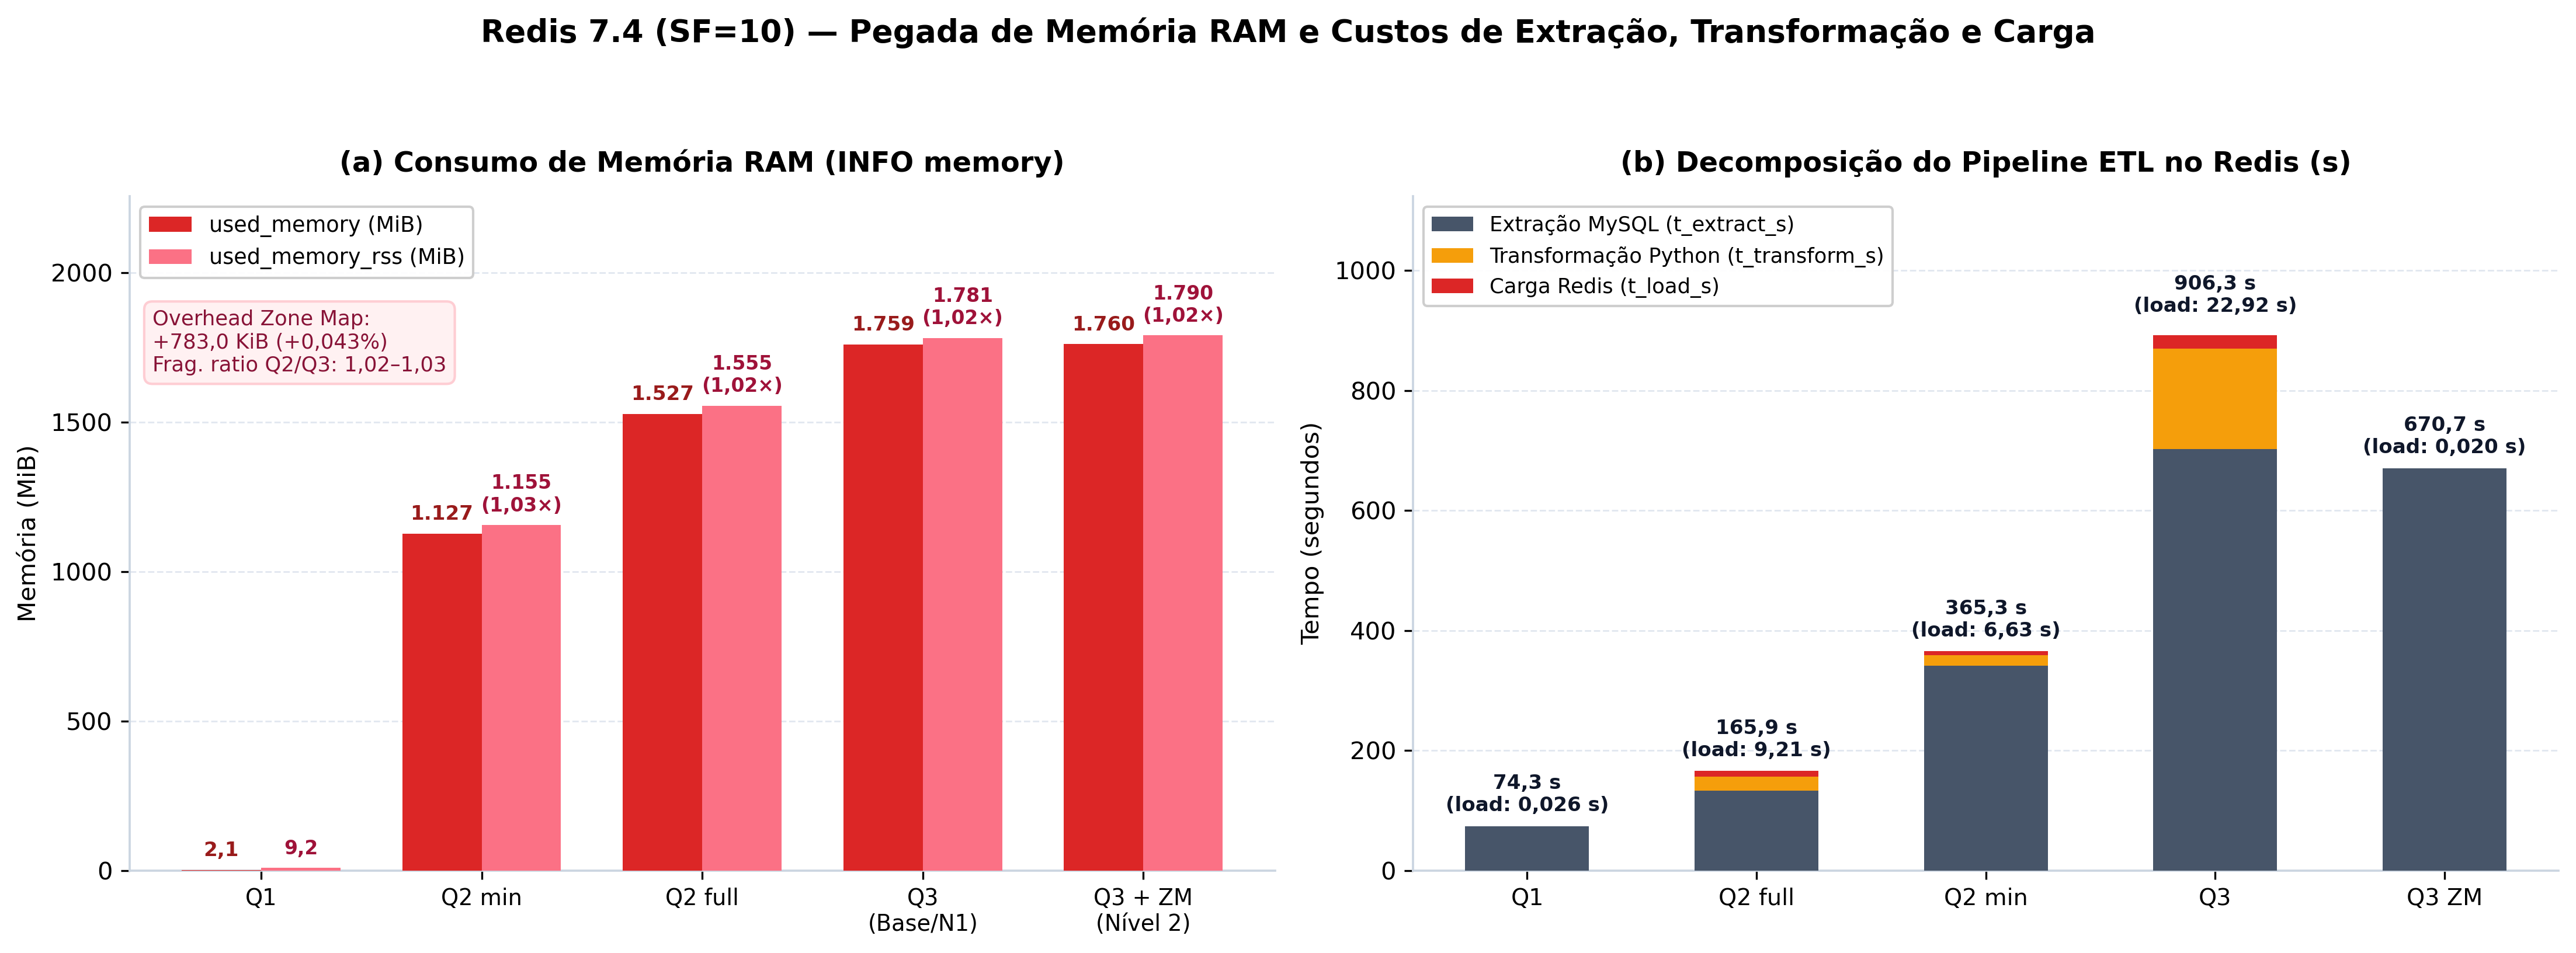
\includegraphics[width=0.95\textwidth]{imagens/Redis/redis_memoria_carga.png}
    \caption{Consumo de memória RAM (\texttt{INFO memory}) e decomposição do pipeline ETL (extração, transformação e carga) no Redis 7.4 em $\text{SF}=10$.}
    \label{fig:redis_mem_etl}
\end{figure}

\begin{figure}[H]
    \centering
    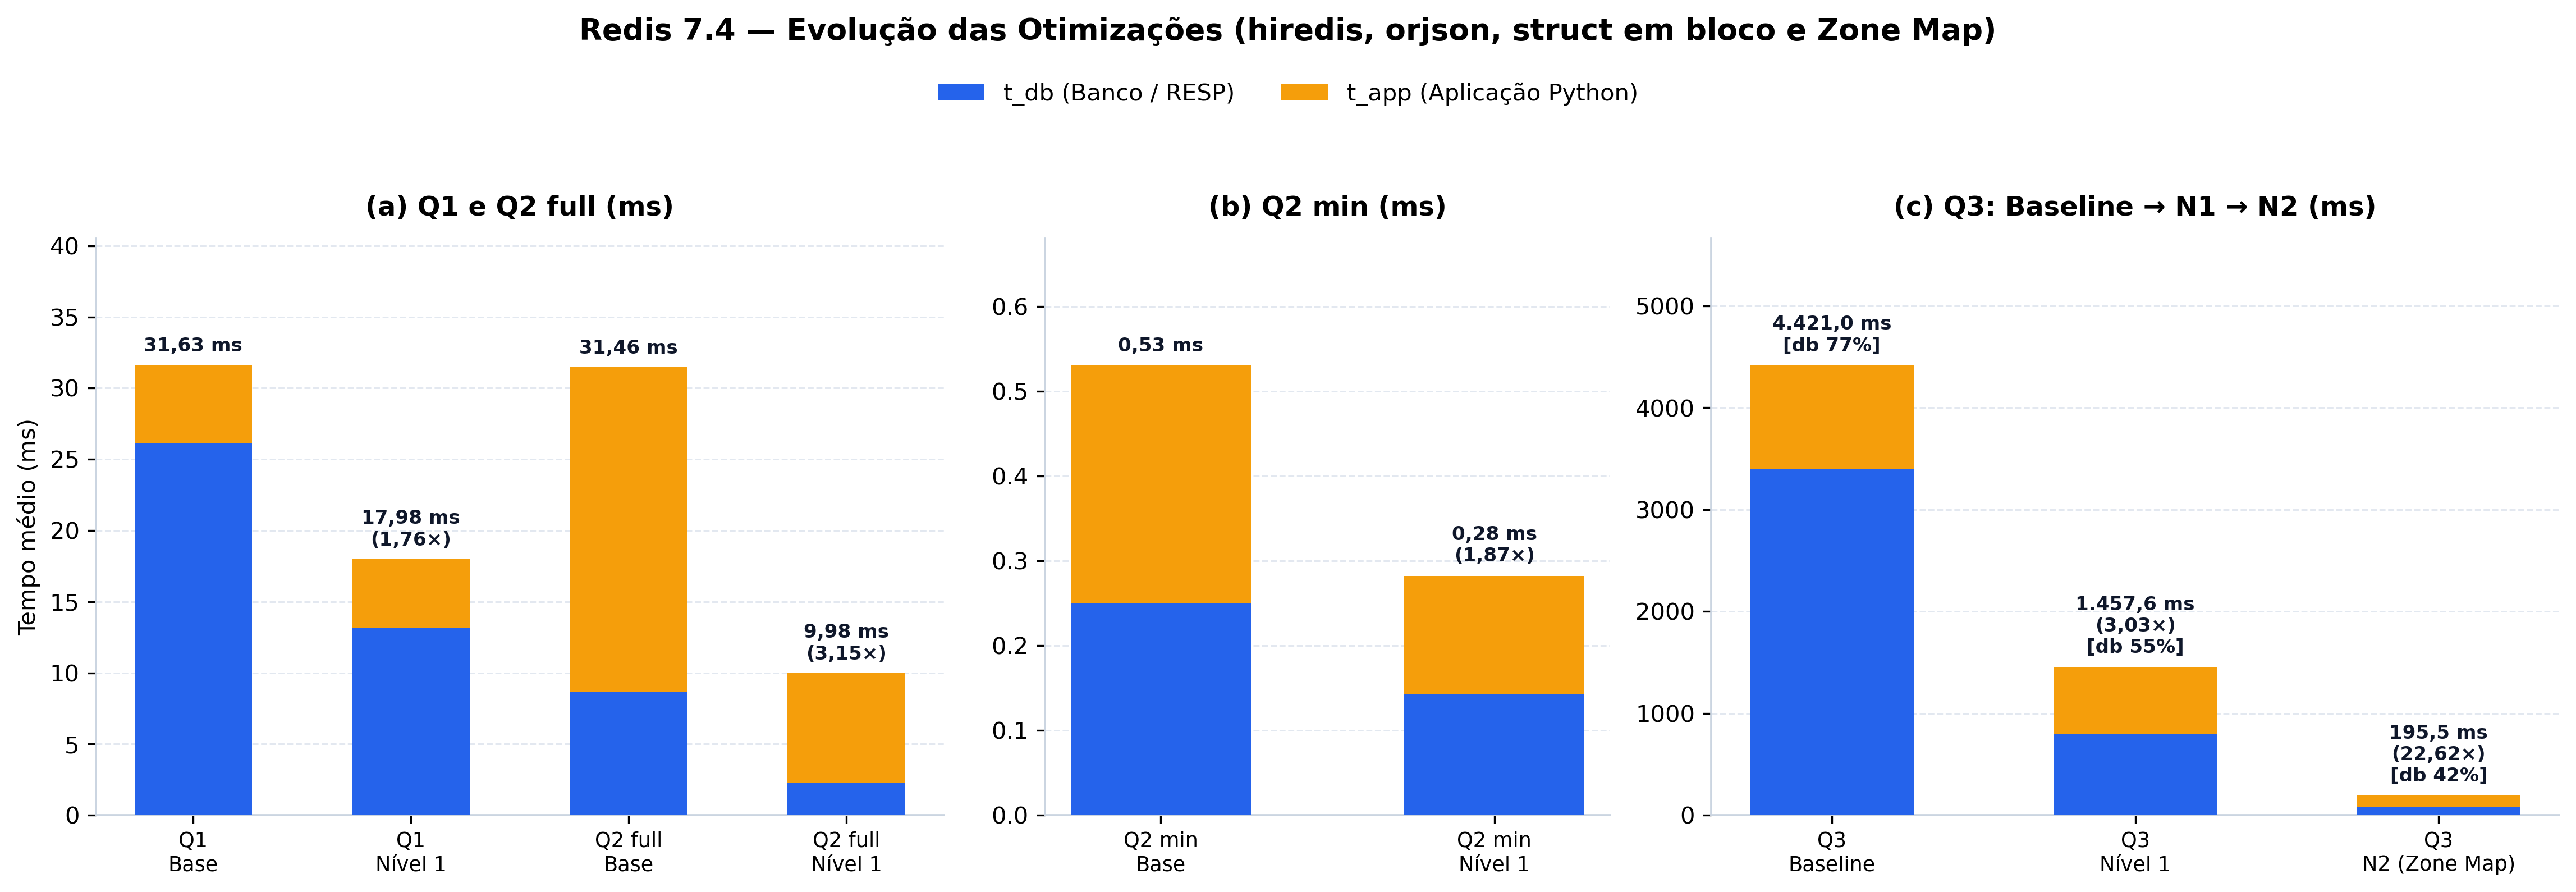
\includegraphics[width=0.95\textwidth]{imagens/Redis/redis_evolucao_otimizacoes.png}
    \caption{Evolução das otimizações no Redis (Base $\rightarrow$ V2 $\rightarrow$ V3 Zone Map; nos gráficos, \textit{Baseline}, \textit{Nível 1} e \textit{Nível 2}) com decomposição \texttt{t\_db} + \texttt{t\_app}.}
    \label{fig:redis_evol}
\end{figure}

\subsection*{Apache Cassandra (Partições, Histogramas e Otimizações)}
\begin{figure}[H]
    \centering
    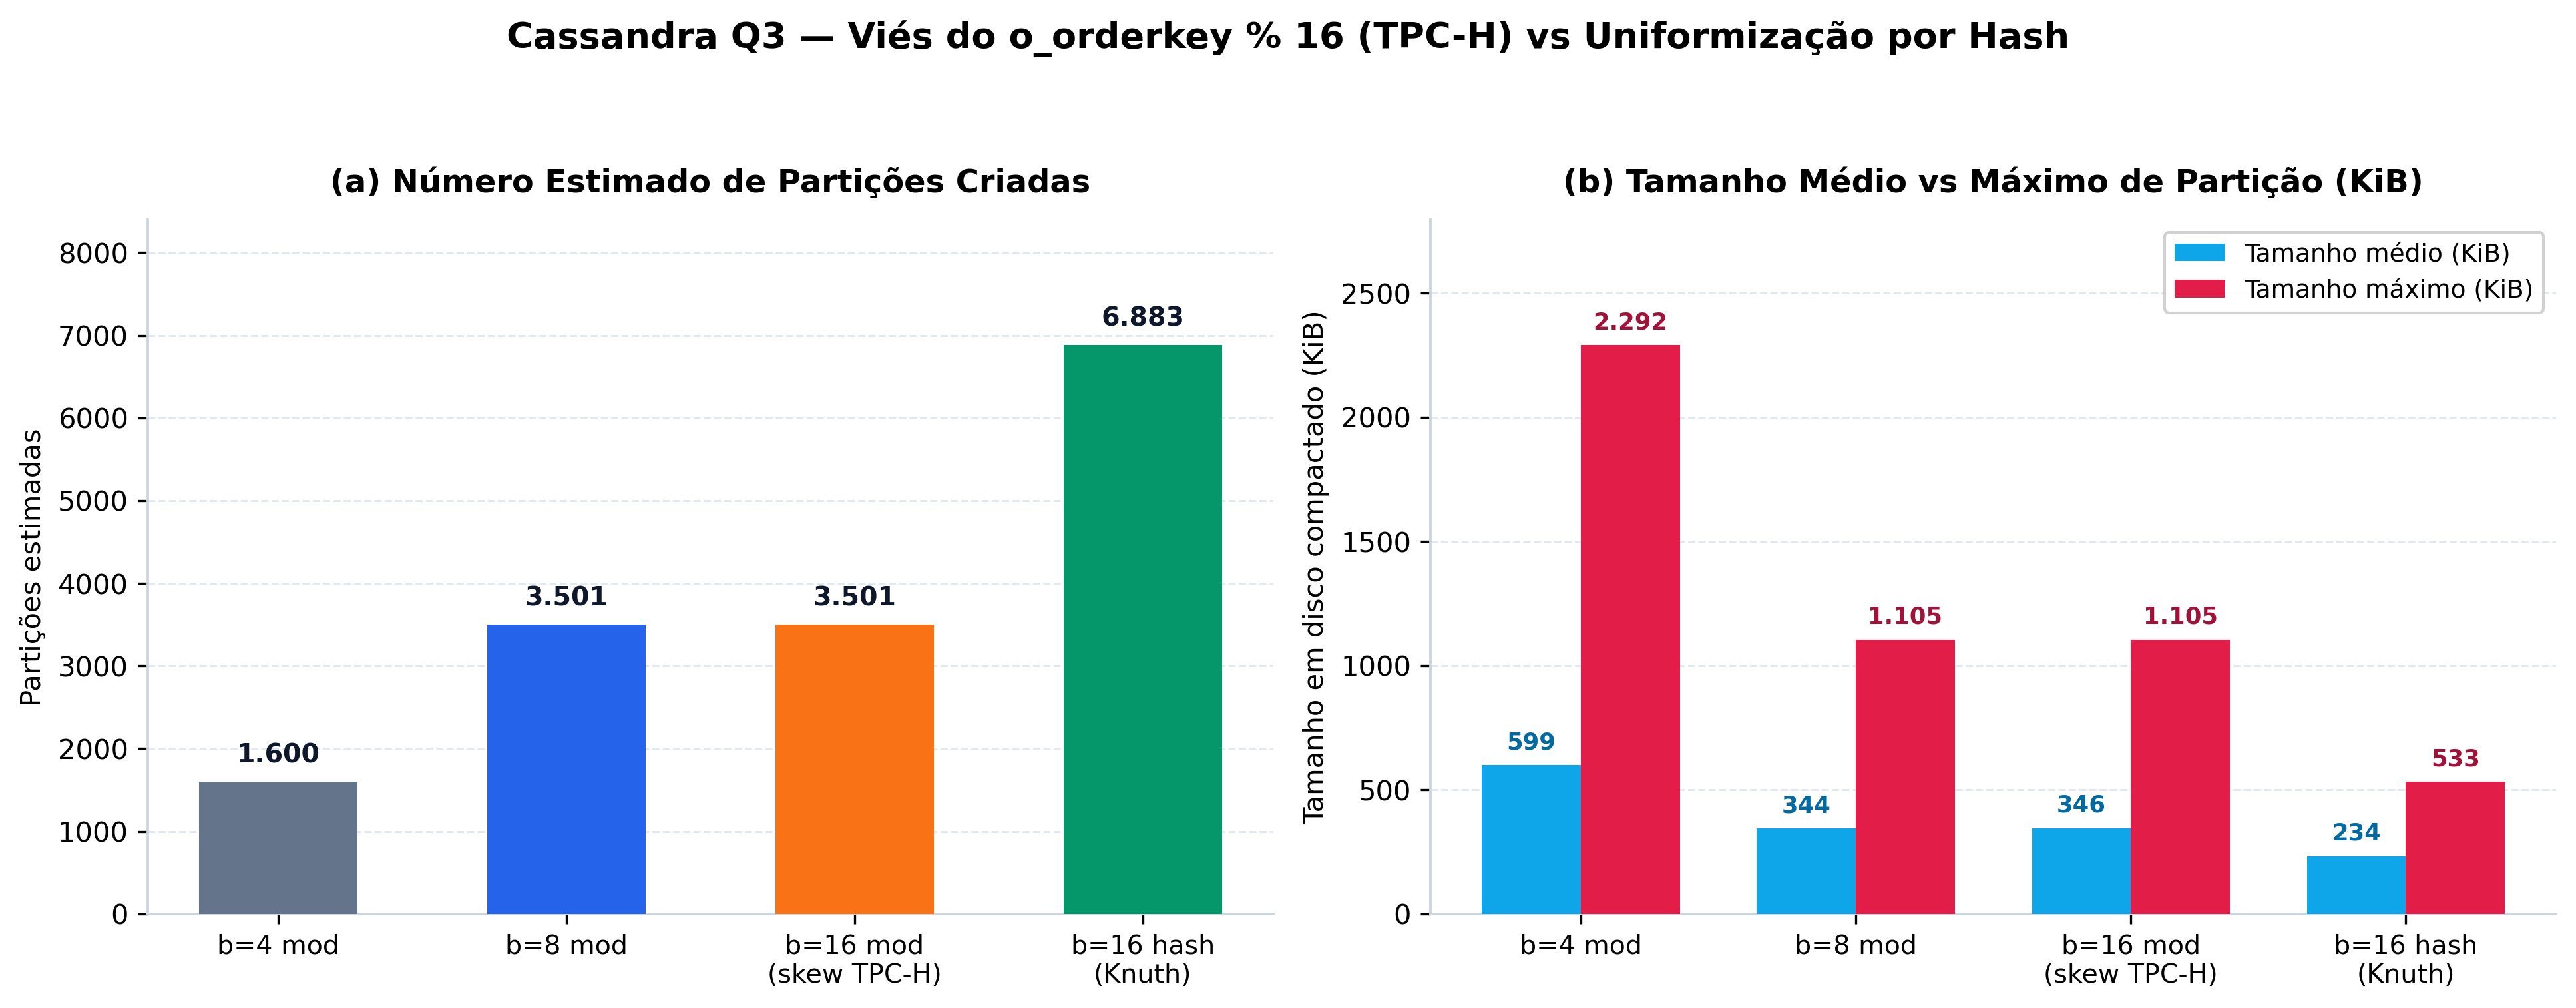
\includegraphics[width=0.95\textwidth]{imagens/Cassandra/fig4_cassandra_partitions.png}
    \caption{Efeito do viés de \texttt{o\_orderkey \% 16} no TPC-H versus uniformização por \textit{hash} de Knuth no número de partições e tamanho médio/máximo.}
    \label{fig:cass_partitions}
\end{figure}

\begin{figure}[H]
    \centering
    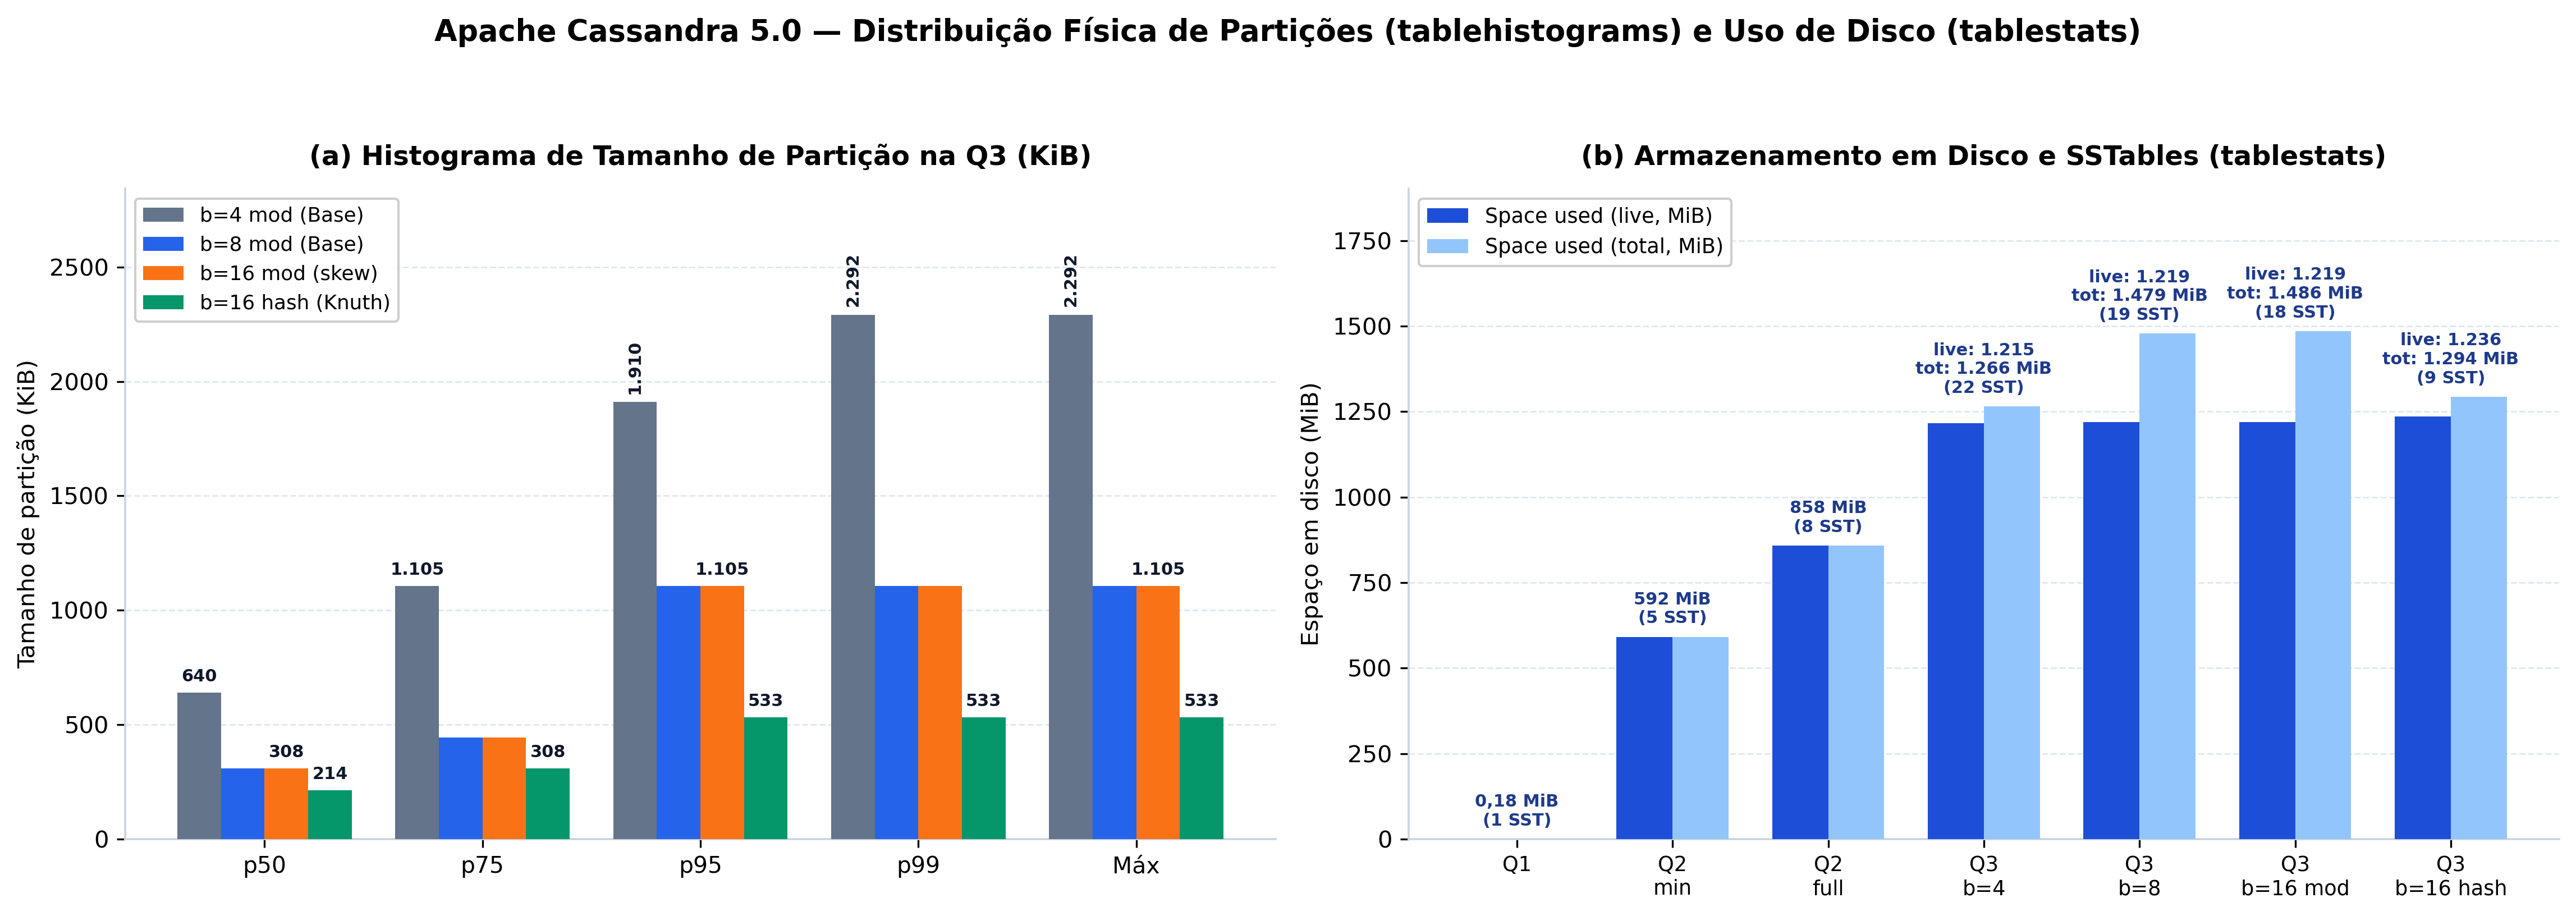
\includegraphics[width=0.95\textwidth]{imagens/Cassandra/cassandra_histograms_q3.png}
    \caption{Distribuição de percentis de tamanho de partição (\texttt{nodetool tablehistograms}) e armazenamento em disco/SSTables (\texttt{nodetool tablestats}) no Cassandra 5.0.}
    \label{fig:cass_histograms}
\end{figure}

\begin{figure}[H]
    \centering
    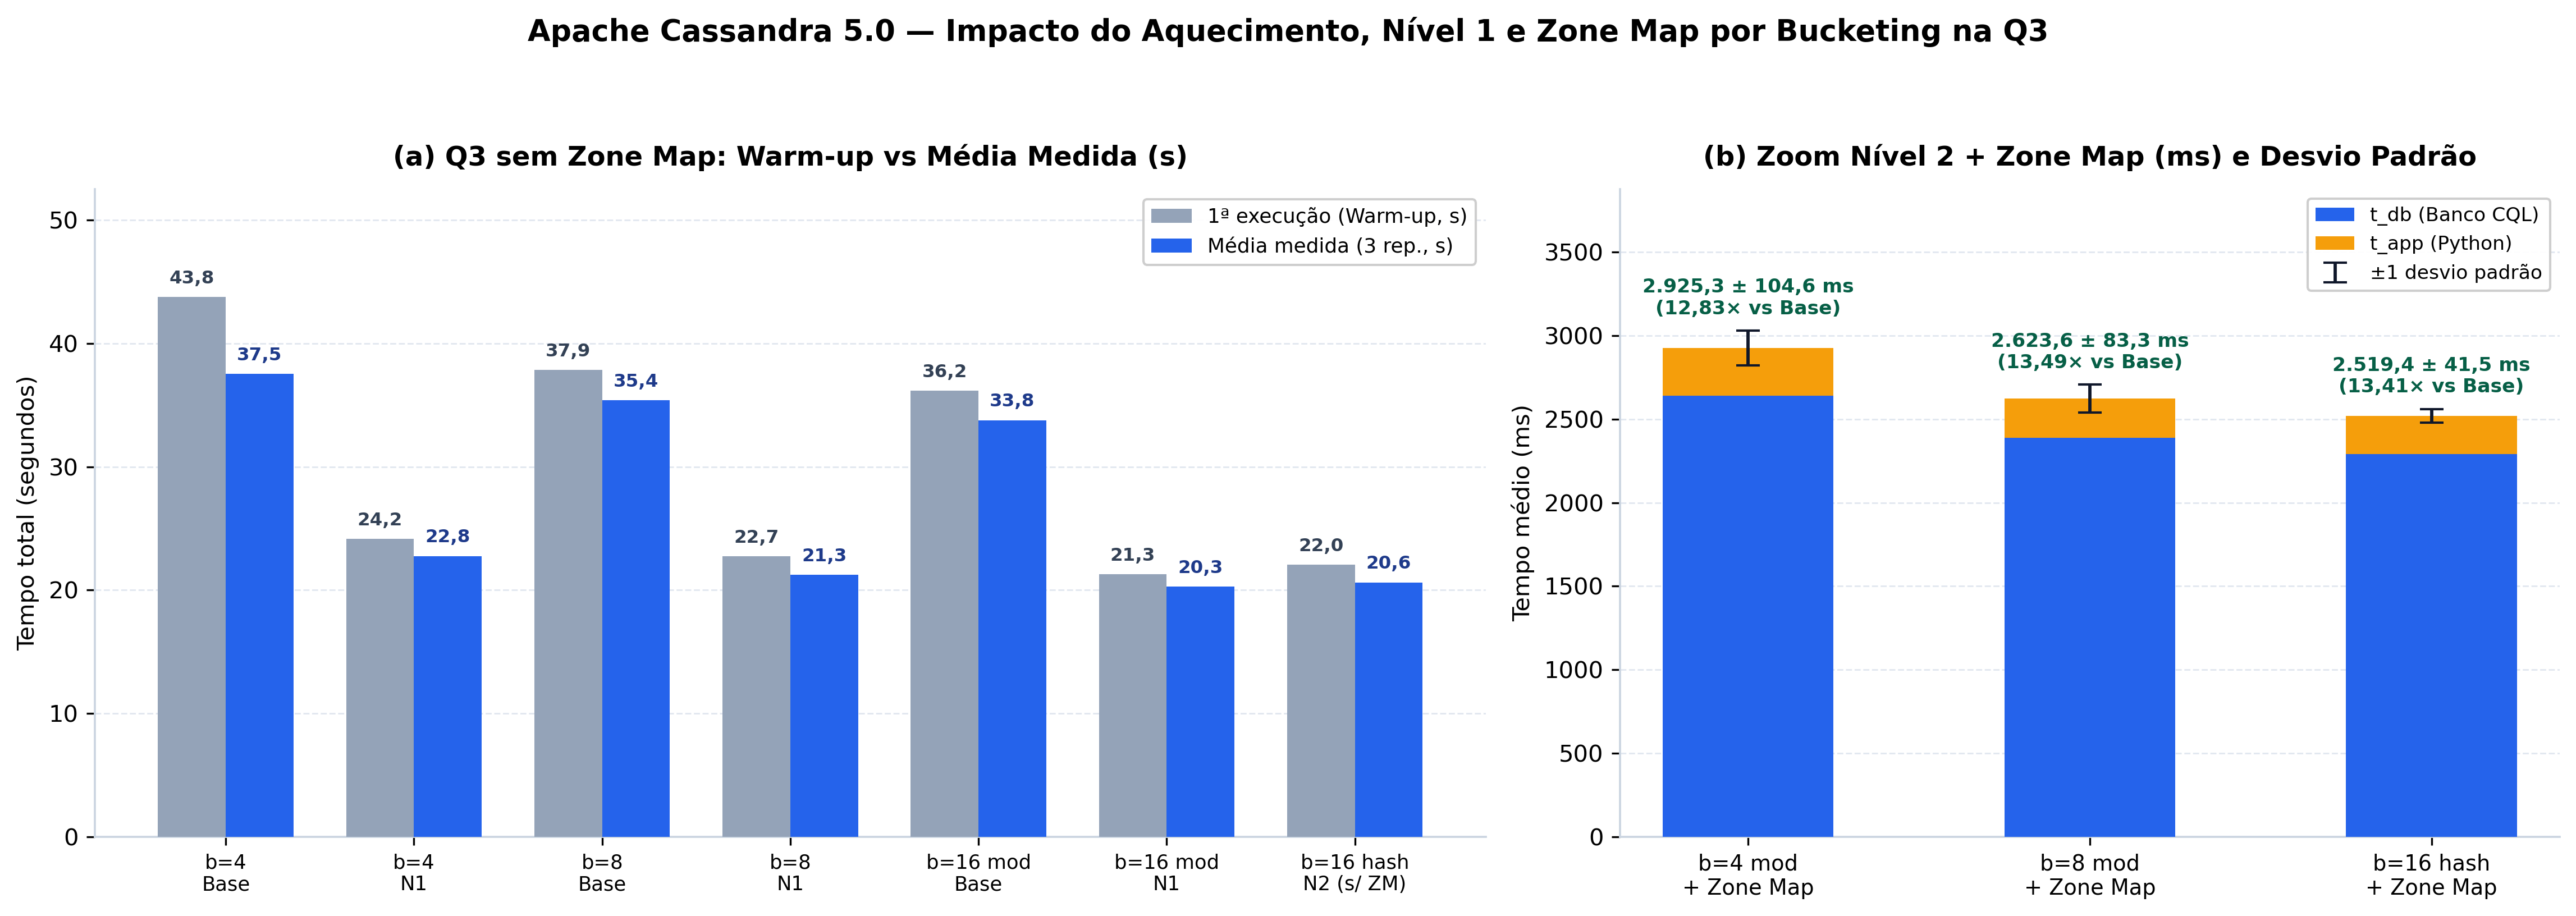
\includegraphics[width=0.95\textwidth]{imagens/Cassandra/cassandra_q3_otimizacoes.png}
    \caption{Impacto do aquecimento (\textit{warm-up}), Versão 2 (\textit{N1}) e Versão 3 + Zone Map (\textit{N2}) na Q3 do Cassandra por configuração de \textit{bucketing}.}
    \label{fig:cass_q3_opt}
\end{figure}

\subsection*{Gráficos Comparativos (Redis vs. Apache Cassandra)}
\begin{figure}[H]
    \centering
    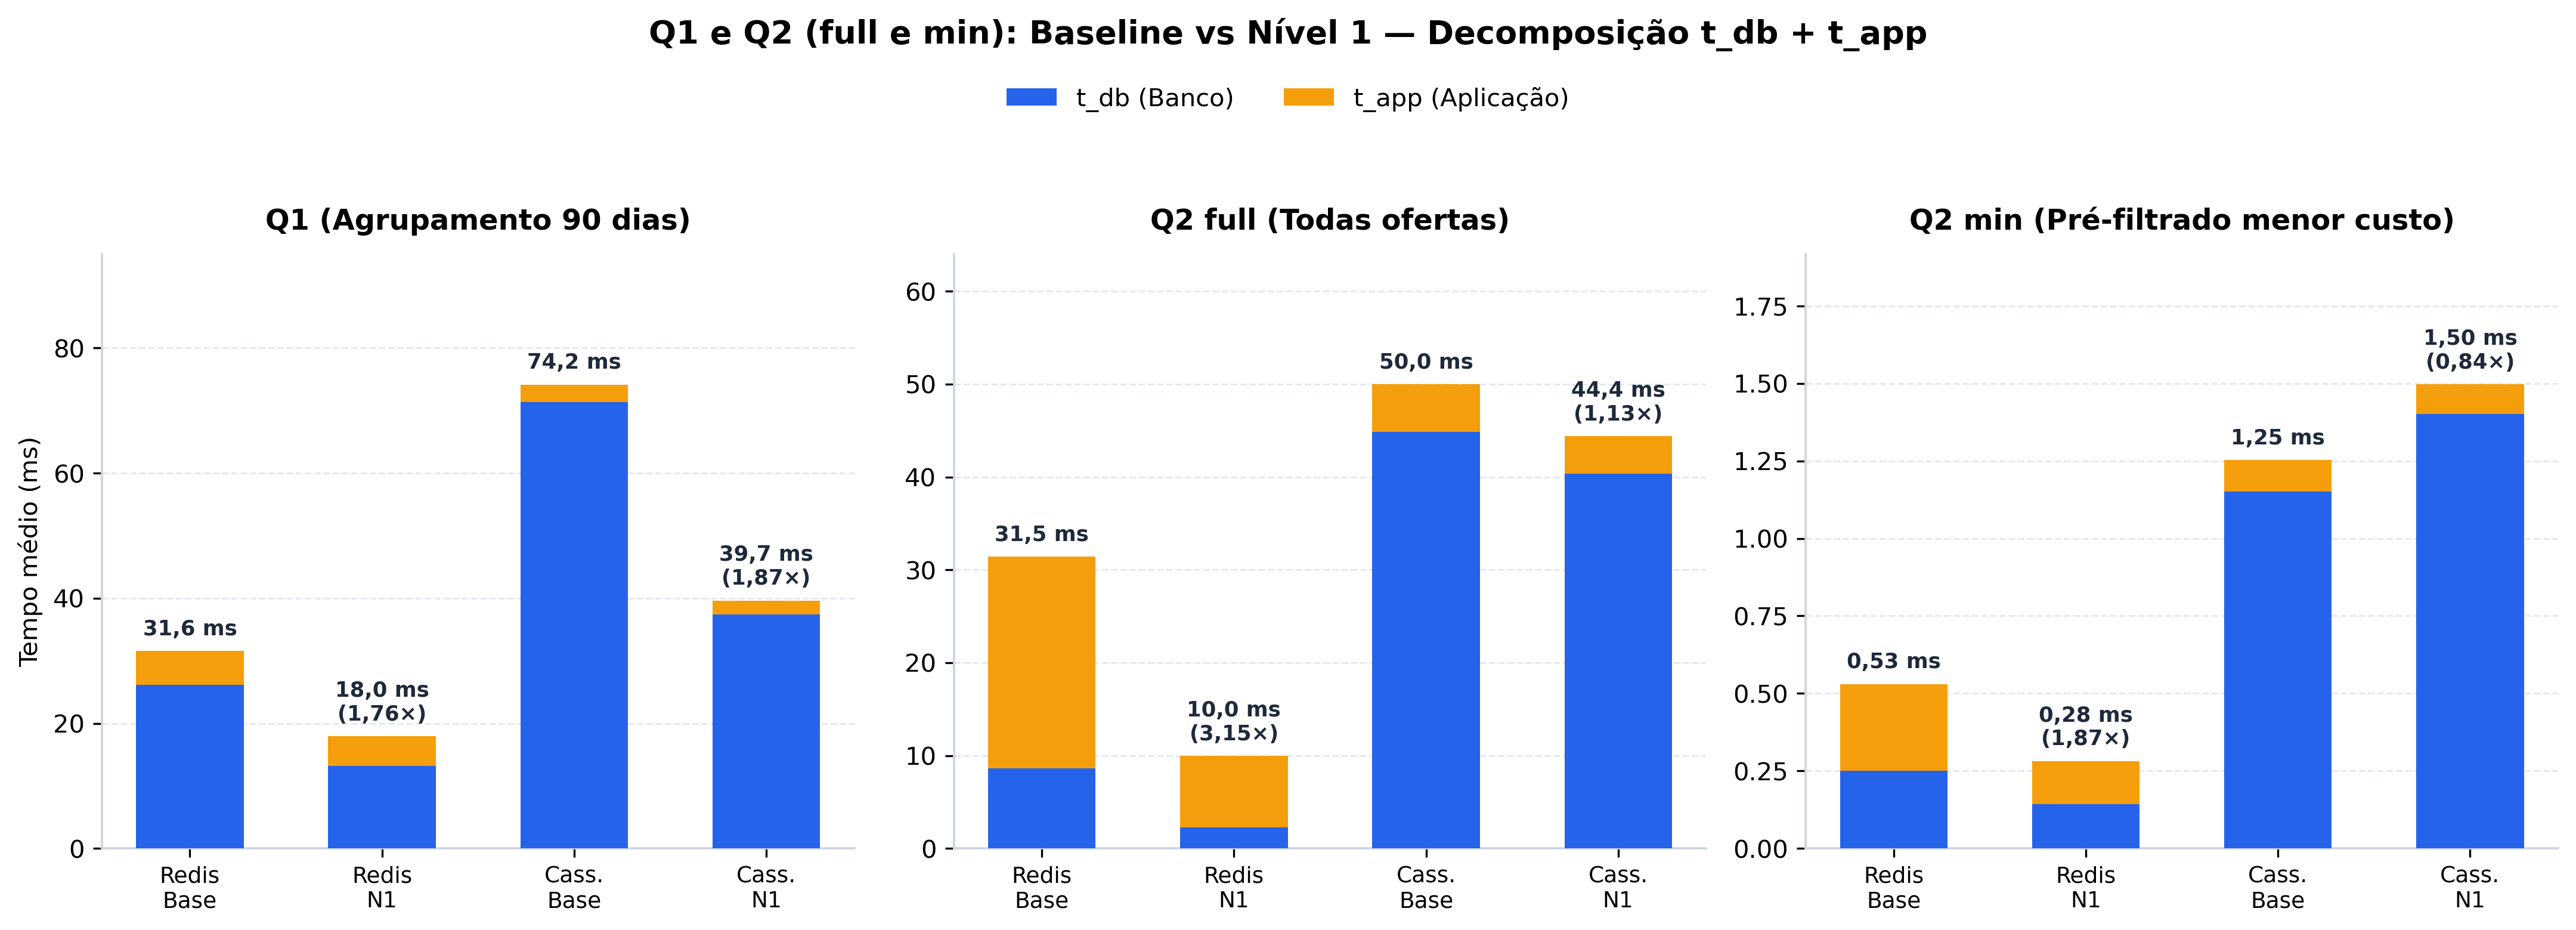
\includegraphics[width=0.95\textwidth]{imagens/fig1_q1_q2_comparison.png}
    \caption{Comparativo de desempenho nas consultas Q1 e Q2 (\texttt{full} e \texttt{min}): Redis vs. Cassandra (Base e Versão 2; rotulados como \textit{Base} e \textit{N1} no gráfico).}
    \label{fig:q1_q2_comp}
\end{figure}

\begin{figure}[H]
    \centering
    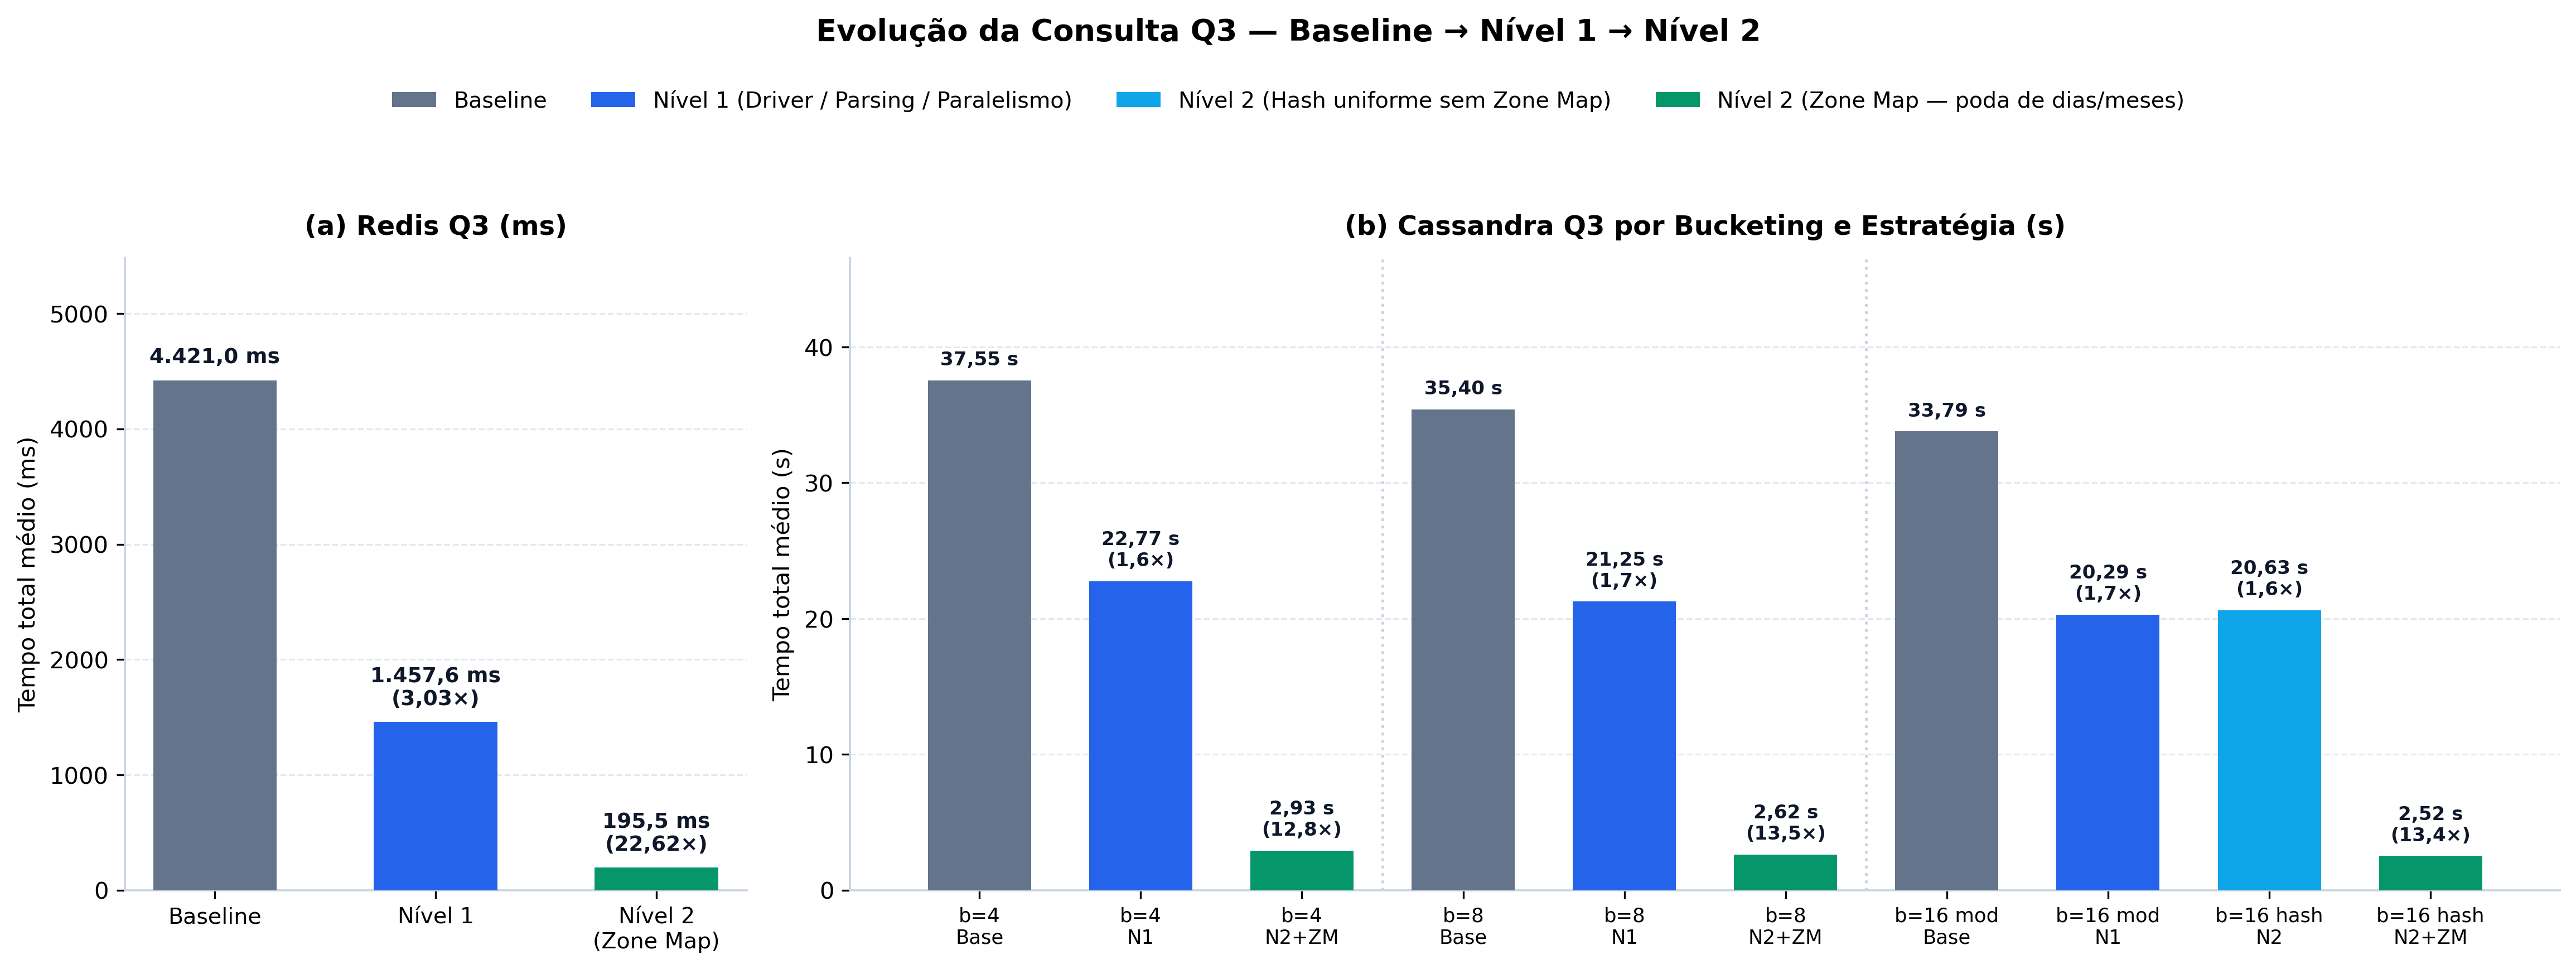
\includegraphics[width=0.95\textwidth]{imagens/fig2_q3_evolution.png}
    \caption{Evolução completa da Query 3 (Base $\rightarrow$ V2 $\rightarrow$ V3; rotulados como \textit{Baseline}, \textit{Nível 1} e \textit{Nível 2} no gráfico) no Redis e no Apache Cassandra.}
    \label{fig:q3_evol}
\end{figure}

\begin{figure}[H]
    \centering
    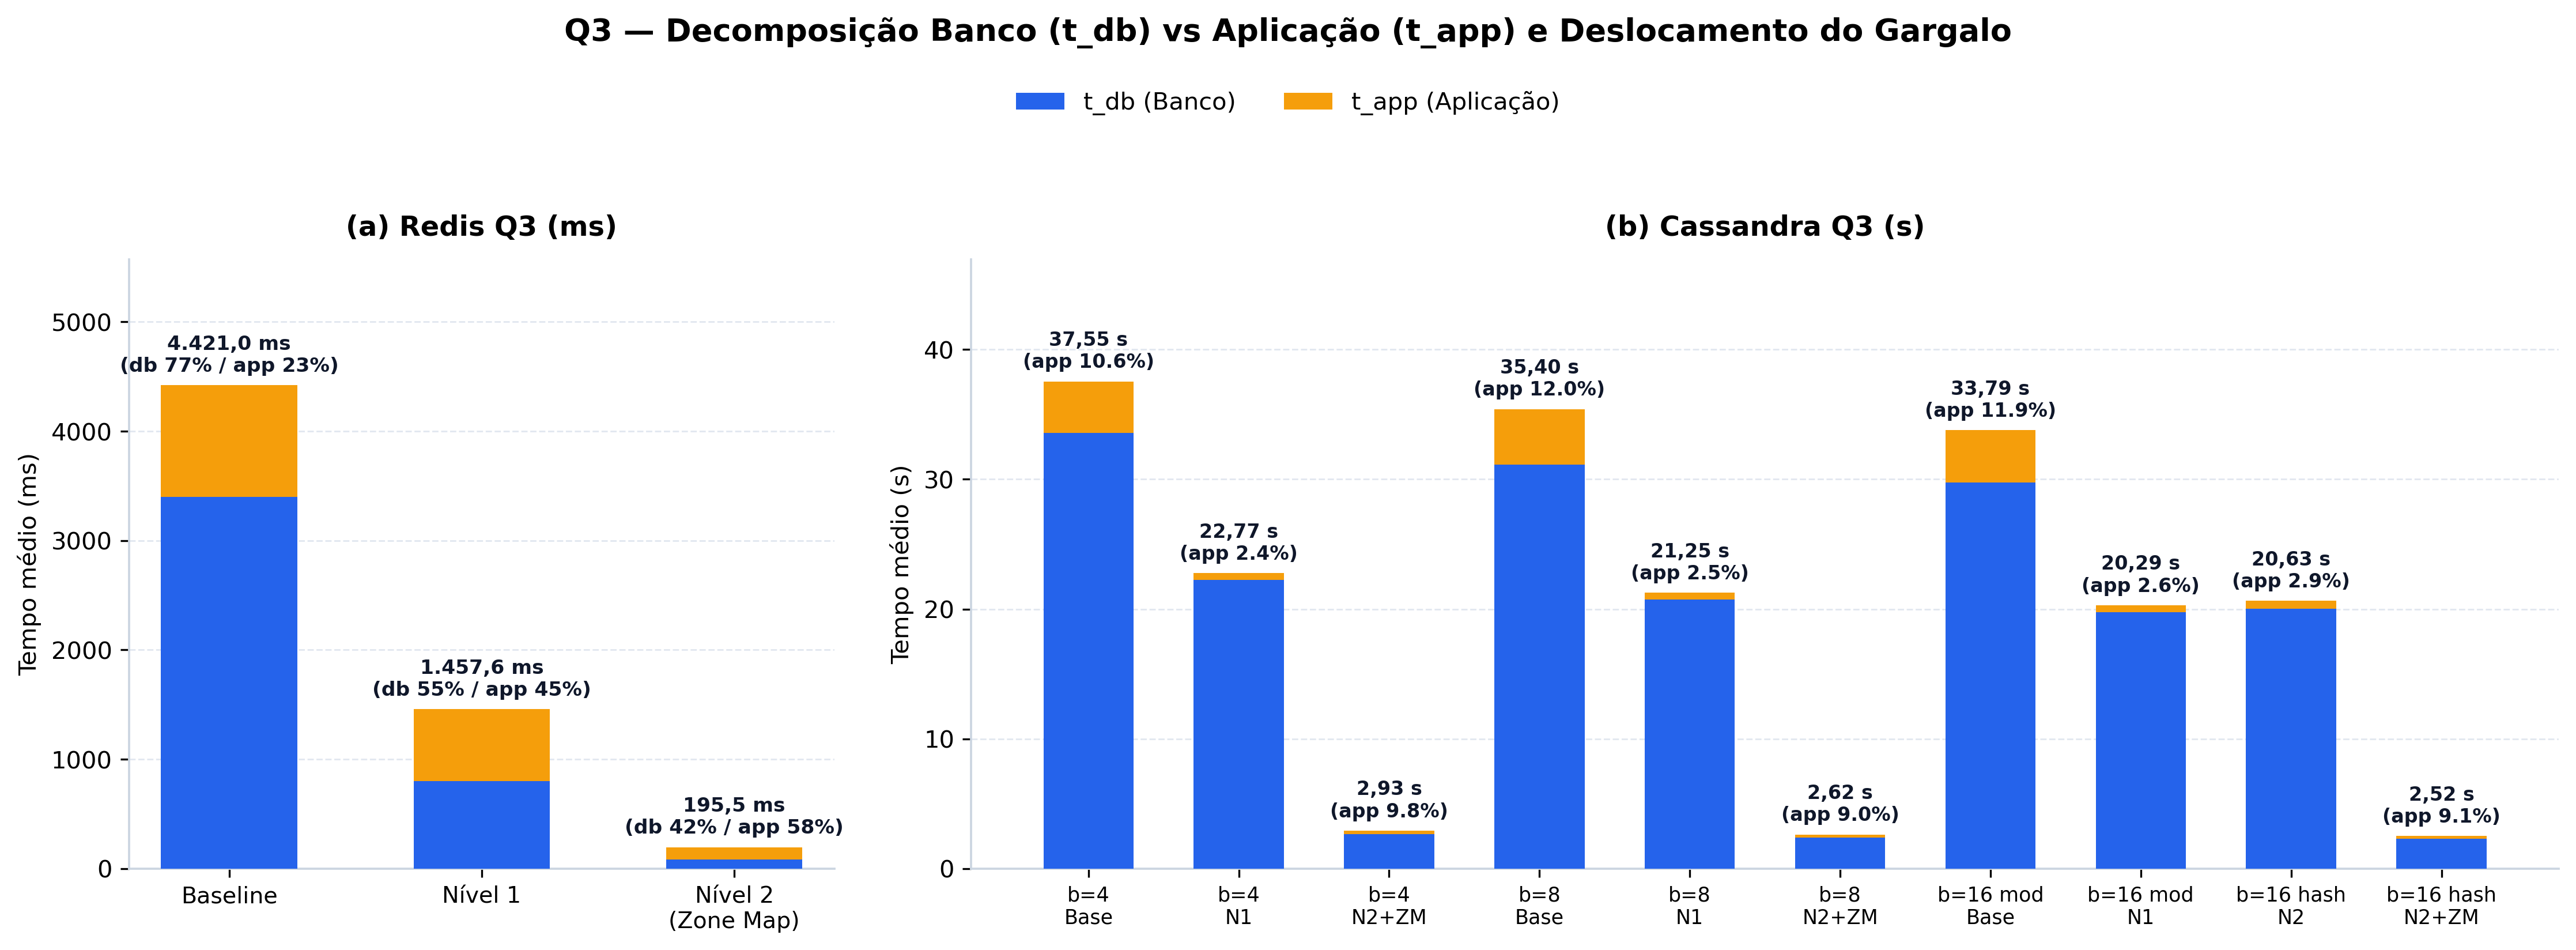
\includegraphics[width=0.95\textwidth]{imagens/fig3_q3_db_vs_app.png}
    \caption{Decomposição \texttt{t\_db} vs. \texttt{t\_app} na Query 3 e deslocamento do gargalo ao longo das otimizações.}
    \label{fig:q3_db_app}
\end{figure}

\begin{figure}[H]
    \centering
    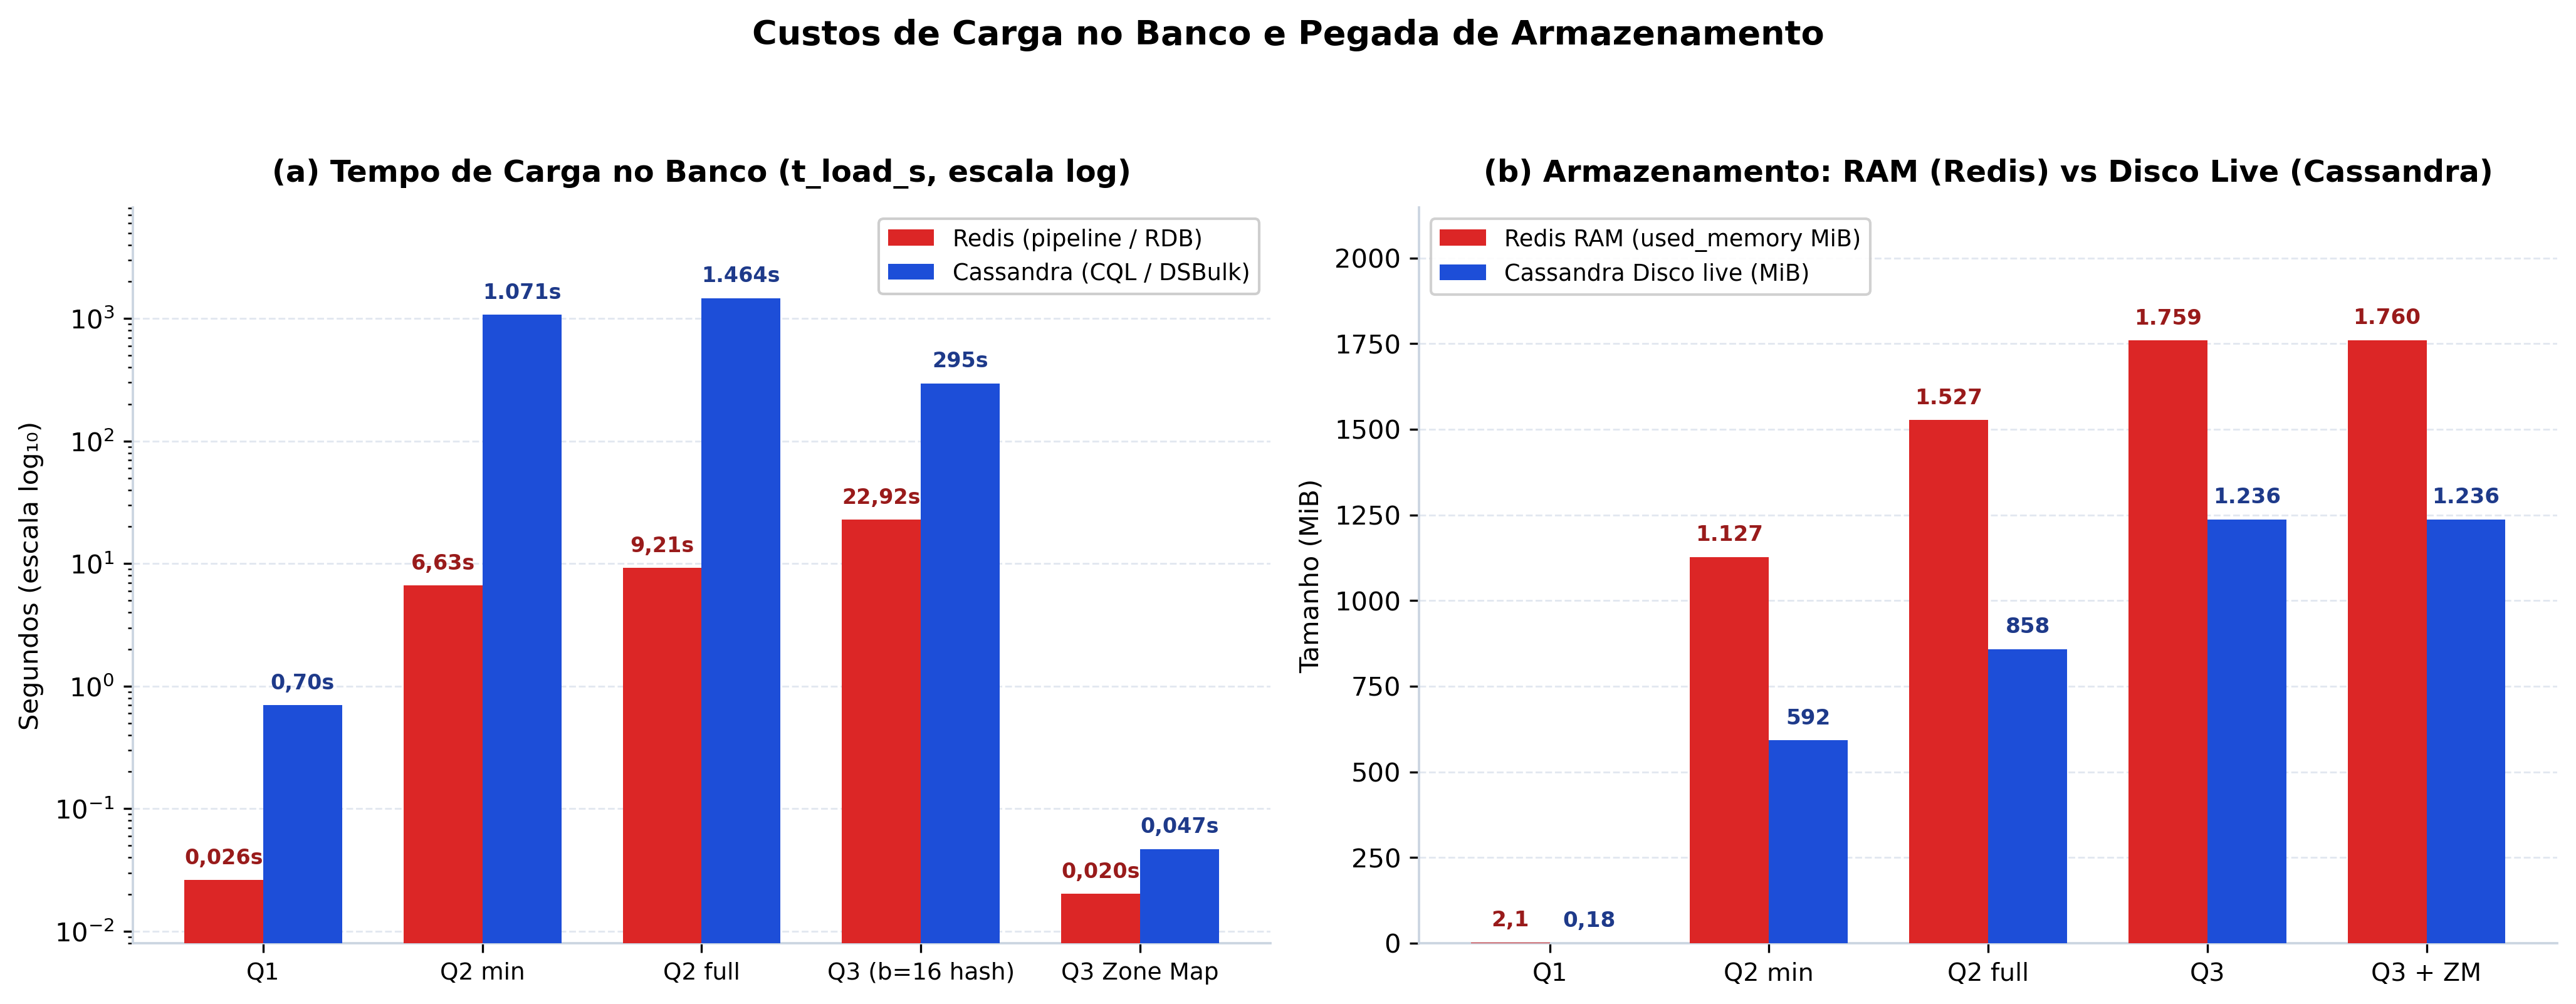
\includegraphics[width=0.95\textwidth]{imagens/fig5_load_and_storage.png}
    \caption{Comparativo de tempo efetivo de carga no banco (\texttt{t\_load\_s}, escala logarítmica) e pegada de armazenamento (RAM vs. disco \textit{live}).}
    \label{fig:load_storage}
\end{figure}

\newpage
\section*{Apêndice A -- Repositório de Código e Reprodutibilidade}
O código-fonte completo utilizado neste estudo --- incluindo os scripts de carga (ETL), as rotinas de execução e validação das três versões (Base, Versão 2 e Versão 3), os \textit{schemas} CQL, os arquivos de configuração Docker e os relatórios JSON de saída --- encontra-se disponível no repositório do projeto:

% Substitua a URL abaixo pelo link real do repositório (GitHub/GitLab)
\begin{center}
\url{https://github.com/SEU-USUARIO/SEU-REPOSITORIO}
\end{center}

\subsection*{Estrutura do Repositório}
Os artefatos do projeto estão organizados em diretórios separados para utilitários compartilhados, Redis e Apache Cassandra, com os scripts de orquestração na raiz:

\begin{lstlisting}[caption={Organização dos arquivos-fonte no repositório do projeto.}]
Projeto2/
|-- docker-compose.yml       # Servicos isolados (tpch_redis e tpch_cassandra)
|-- cassandra.yaml           # Configuracao personalizada de timeouts do servidor
|-- schema.cql               # Schema CQL inicial (Base)
|-- schema_opt.cql           # Schema CQL adicional da V3 (tabela q3_zonemap)
|-- mysql_result.py          # Geracao do gabarito JSON a partir do MySQL (SF=10)
|-- script.sh                # Orquestracao completa da versao Base
|-- run_opt_nivel1.sh        # Orquestracao da Versao 2 (camada cliente)
|-- run_opt_nivel2.sh        # Orquestracao da Versao 3 (Zone Maps + hash Knuth)
|-- generate_report.py       # Consolidacao dos JSONs, tabelas e graficos
|-- common/
|   |-- config.py            # Caminhos dinamicos e fabricas de conexao
|   |-- codecs.py            # Empacotamento binario struct da Q3 e chaves Redis
|   `-- test_runner.py       # Executor padronizado de warmup, repeticoes e validacao
|-- Redis/
|   |-- load/                # load_q1.py, load_q2.py, load_q3.py
|   |-- test/                # test_q1.py, test_q2.py, test_q3.py (Base)
|   |-- opt/                 # load_q3_zonemap.py e test_*_opt.py (V2 e V3)
|   |-- run_load_backup.sh   # Carga isolada e snapshot RDB sincrono (SAVE)
|   `-- run_test_from_backup.sh
`-- Cassandra/
    |-- load/                # load_q1.py, load_q2.py, export_q3_csv.py, load_q3_dsbulk.sh
    |-- test/                # test_q1.py, test_q2.py, test_q3.py (Base)
    `-- opt/                 # load_q3_zonemap.py, test_*_opt.py (V2) e test_q3_nivel2.py (V3)
\end{lstlisting}

\subsection*{Comandos de Reprodutibilidade}
Tendo o MySQL populado com a base TPC-H ($\text{SF}=10$), o Docker Compose ativo e o binário do DataStax Bulk Loader (\texttt{dsbulk} 1.11.0) disponível no \texttt{PATH} (ou no diretório \texttt{dsbulk-1.11.0/bin}), as três baterias experimentais podem ser reproduzidas em sequência a partir da raiz do repositório:

\begin{lstlisting}[caption={Sequência de comandos para preparar o ambiente e reproduzir Base, Versão 2 e Versão 3.}]
python3 -m venv .venv && source .venv/bin/activate
pip install mysql-connector-python redis hiredis orjson cassandra-driver
export MYSQL_PASSWORD="sua_senha_mysql"

# 1. Versao Base: gabarito MySQL, carga e testes (Redis e Cassandra)
./script.sh all

# 2. Versao 2 (camada cliente: hiredis/orjson e execute_async; script run_opt_nivel1.sh)
./run_opt_nivel1.sh all

# 3. Versao 3 (Zone Maps na Q3 e hash de Knuth em b=16; script run_opt_nivel2.sh)
./run_opt_nivel2.sh all
\end{lstlisting}

\end{document}
